\documentclass[a4paper,12pt,twoside]{memoir}

% Castellano
\usepackage[spanish,es-tabla]{babel}
\selectlanguage{spanish}
\usepackage[utf8]{inputenc}
\usepackage[T1]{fontenc}
\usepackage{lmodern} % Scalable font
\usepackage{microtype}
\usepackage{placeins}
\usepackage{multicol}
\usepackage{booktabs} % Para mejorar la apariencia de las tablas
\usepackage{longtable}
\usepackage{adjustbox}
\usepackage{dirtree}
\usepackage{float}
\usepackage{listings}
\usepackage[hyphens]{url}

\lstset{
    basicstyle=\ttfamily,
    breaklines=true,
    escapeinside={(*@}{@*)},
    xleftmargin=0pt,
    xrightmargin=0pt,
    showstringspaces=false % Opcional: no muestra espacios especiales en cadenas
}

\RequirePackage{booktabs}
\RequirePackage[table]{xcolor}
\RequirePackage{xtab}
\RequirePackage{multirow}

% Links
\usepackage[colorlinks]{hyperref}
\hypersetup{
	allcolors = {red}
}

% Ecuaciones
\usepackage{amsmath}

% Rutas de fichero / paquete
\newcommand{\ruta}[1]{{\sffamily #1}}

% Párrafos
\nonzeroparskip

% Huérfanas y viudas
\widowpenalty100000
\clubpenalty100000

% Evitar solapes en el header
\nouppercaseheads

% Imagenes
\usepackage{graphicx}
\newcommand{\imagen}[2]{
	\begin{figure}[!h]
		\centering
		\includegraphics[width=0.9\textwidth]{#1}
		\caption{#2}\label{fig:#1}
	\end{figure}
	\FloatBarrier
}

\newcommand{\imagenflotante}[2]{
	\begin{figure}%[!h]
		\centering
		\includegraphics[width=0.9\textwidth]{#1}
		\caption{#2}\label{fig:#1}
	\end{figure}
}



% El comando \figura nos permite insertar figuras comodamente, y utilizando
% siempre el mismo formato. Los parametros son:
% 1 -> Porcentaje del ancho de página que ocupará la figura (de 0 a 1)
% 2 --> Fichero de la imagen
% 3 --> Texto a pie de imagen
% 4 --> Etiqueta (label) para referencias
% 5 --> Opciones que queramos pasarle al \includegraphics
% 6 --> Opciones de posicionamiento a pasarle a \begin{figure}
\newcommand{\figuraConPosicion}[6]{%
  \setlength{\anchoFloat}{#1\textwidth}%
  \addtolength{\anchoFloat}{-4\fboxsep}%
  \setlength{\anchoFigura}{\anchoFloat}%
  \begin{figure}[#6]
    \begin{center}%
      \Ovalbox{%
        \begin{minipage}{\anchoFloat}%
          \begin{center}%
            \includegraphics[width=\anchoFigura,#5]{#2}%
            \caption{#3}%
            \label{#4}%
          \end{center}%
        \end{minipage}
      }%
    \end{center}%
  \end{figure}%
}

%
% Comando para incluir imágenes en formato apaisado (sin marco).
\newcommand{\figuraApaisadaSinMarco}[5]{%
  \begin{figure}%
    \begin{center}%
    \includegraphics[angle=90,height=#1\textheight,#5]{#2}%
    \caption{#3}%
    \label{#4}%
    \end{center}%
  \end{figure}%
}
% Para las tablas
\newcommand{\otoprule}{\midrule [\heavyrulewidth]}
%
% Nuevo comando para tablas pequeñas (menos de una página).
\newcommand{\tablaSmall}[5]{%
 \begin{table}
  \begin{center}
   \rowcolors {2}{gray!35}{}
   \begin{tabular}{#2}
    \toprule
    #4
    \otoprule
    #5
    \bottomrule
   \end{tabular}
   \caption{#1}
   \label{tabla:#3}
  \end{center}
 \end{table}
}

%
% Nuevo comando para tablas pequeñas (menos de una página).
\newcommand{\tablaSmallSinColores}[5]{%
 \begin{table}[H]
  \begin{center}
   \begin{tabular}{#2}
    \toprule
    #4
    \otoprule
    #5
    \bottomrule
   \end{tabular}
   \caption{#1}
   \label{tabla:#3}
  \end{center}
 \end{table}
}

\newcommand{\tablaApaisadaSmall}[5]{%
\begin{landscape}
  \begin{table}
   \begin{center}
    \rowcolors {2}{gray!35}{}
    \begin{tabular}{#2}
     \toprule
     #4
     \otoprule
     #5
     \bottomrule
    \end{tabular}
    \caption{#1}
    \label{tabla:#3}
   \end{center}
  \end{table}
\end{landscape}
}

%
% Nuevo comando para tablas grandes con cabecera y filas alternas coloreadas en gris.
\newcommand{\tabla}[6]{%
  \begin{center}
    \tablefirsthead{
      \toprule
      #5
      \otoprule
    }
    \tablehead{
      \multicolumn{#3}{l}{\small\sl continúa desde la página anterior}\\
      \toprule
      #5
      \otoprule
    }
    \tabletail{
      \hline
      \multicolumn{#3}{r}{\small\sl continúa en la página siguiente}\\
    }
    \tablelasttail{
      \hline
    }
    \bottomcaption{#1}
    \rowcolors {2}{gray!35}{}
    \begin{xtabular}{#2}
      #6
      \bottomrule
    \end{xtabular}
    \label{tabla:#4}
  \end{center}
}

%
% Nuevo comando para tablas grandes con cabecera.
\newcommand{\tablaSinColores}[6]{%
  \begin{center}
    \tablefirsthead{
      \toprule
      #5
      \otoprule
    }
    \tablehead{
      \multicolumn{#3}{l}{\small\sl continúa desde la página anterior}\\
      \toprule
      #5
      \otoprule
    }
    \tabletail{
      \hline
      \multicolumn{#3}{r}{\small\sl continúa en la página siguiente}\\
    }
    \tablelasttail{
      \hline
    }
    \bottomcaption{#1}
    \begin{xtabular}{#2}
      #6
      \bottomrule
    \end{xtabular}
    \label{tabla:#4}
  \end{center}
}

%
% Nuevo comando para tablas grandes sin cabecera.
\newcommand{\tablaSinCabecera}[5]{%
  \begin{center}
    \tablefirsthead{
      \toprule
    }
    \tablehead{
      \multicolumn{#3}{l}{\small\sl continúa desde la página anterior}\\
      \hline
    }
    \tabletail{
      \hline
      \multicolumn{#3}{r}{\small\sl continúa en la página siguiente}\\
    }
    \tablelasttail{
      \hline
    }
    \bottomcaption{#1}
  \begin{xtabular}{#2}
    #5
   \bottomrule
  \end{xtabular}
  \label{tabla:#4}
  \end{center}
}



\definecolor{cgoLight}{HTML}{EEEEEE}
\definecolor{cgoExtralight}{HTML}{FFFFFF}

%
% Nuevo comando para tablas grandes sin cabecera.
\newcommand{\tablaSinCabeceraConBandas}[5]{%
  \begin{center}
    \tablefirsthead{
      \toprule
    }
    \tablehead{
      \multicolumn{#3}{l}{\small\sl continúa desde la página anterior}\\
      \hline
    }
    \tabletail{
      \hline
      \multicolumn{#3}{r}{\small\sl continúa en la página siguiente}\\
    }
    \tablelasttail{
      \hline
    }
    \bottomcaption{#1}
    \rowcolors[]{1}{cgoExtralight}{cgoLight}

  \begin{xtabular}{#2}
    #5
   \bottomrule
  \end{xtabular}
  \label{tabla:#4}
  \end{center}
}


\graphicspath{ {./img/} }

% Capítulos
\chapterstyle{bianchi}
\newcommand{\capitulo}[2]{
	\setcounter{chapter}{#1}
	\setcounter{section}{0}
	\chapter*{#2}
	\addcontentsline{toc}{chapter}{#1. #2}
	\markboth{#2}{#2}
}

% Apéndices
\renewcommand{\appendixname}{Apéndice}
\renewcommand*\cftappendixname{\appendixname}

\newcommand{\apendice}[1]{
	%\renewcommand{\thechapter}{A}
	\chapter{#1}
}

\renewcommand*\cftappendixname{\appendixname\ }

% Formato de portada
\makeatletter
\usepackage{xcolor}
\newcommand{\tutor}[1]{\def\@tutor{#1}}
\newcommand{\tutorb}[1]{\def\@tutorb{#1}}
\newcommand{\course}[1]{\def\@course{#1}}
\definecolor{cpardoBox}{HTML}{E6E6FF}
\def\maketitle{
  \null
  \thispagestyle{empty}
  % Cabecera ----------------
\begin{center}%
	{\noindent\Huge Universidades de Burgos, León y Valladolid}\vspace{.5cm}%

	{\noindent\Large Máster universitario}\vspace{.5cm}%

	{\noindent\Huge \textbf{Inteligencia de Negocio y Big~Data en Entornos Seguros}}\vspace{.5cm}%
\end{center}%

\begin{center}%
	\includegraphics[height=3cm]{img/escudoUBU} \hspace{1cm}
	\includegraphics[height=3cm]{img/escudoUVA} \hspace{1cm}
	\includegraphics[height=3cm]{img/escudoULE} \vspace{1cm}%
\end{center}%

  \vfill
  % Título proyecto y escudo informática ----------------
  \colorbox{cpardoBox}{%
    \begin{minipage}{.9\textwidth}
      \vspace{.2cm}\Large
      \begin{center}
      \textbf{TFM del Máster Inteligencia de Negocio y Big Data en Entornos Seguros}\vspace{.6cm}\\
      \textbf{\LARGE\@title{}}
      \end{center}
      \vspace{.2cm}
    \end{minipage}

  }%
  \hfill
  \vfill
  % Datos de alumno, curso y tutores ------------------
  \begin{center}%
  {%
    \noindent\large
    Presentado por \@author{}\\
    en Universidad de Burgos a \\ \@date{}\\
    Tutor: \@tutor{}\\
    Co-tutor: \@tutorb{}\\
  }%
  \end{center}%
  \null
  \cleardoublepage
  }
\makeatother

\newcommand{\nombre}{Nombre del alumno} %%% cambio de comando

% Datos de portada
\title{Flujo de Datos para Descubrimiento de Oportunidades Inmobiliarias}
\author{David Puerta Martos}
\tutor{Álvar Arnaiz González}
\tutorb{José Antonio Barbero Aparicio}
\date{\today}

\begin{document}

\maketitle


\frontmatter

% Abstract en castellano
\renewcommand*\abstractname{Resumen}
\begin{abstract}
En este proyecto se ha desarrollado un proceso de extracción, transformación y carga de datos inmobiliarios, obtenidos desde uno de los portales más destacados de España, \href{https://www.pisos.com}{pisos.com}. Este proceso se complementa con el análisis de los datos mediante técnicas de Aprendizaje Automático, con el objetivo de descubrir potenciales oportunidades de compra de inmuebles. 

Como resultado, se ha creado una interfaz web accesible en \href{https://www.buscahogar.es}{www.buscahogar.es}, que permite a los usuarios filtrar, buscar y ordenar inmuebles disponibles según el valor asignado por los modelos, además de otras características, ofreciendo así una herramienta poderosa para potenciales compradores. También, se ofrece la posibilidad de visualizar datos agregados de todo el mercado inmobiliario, filtrados y segmentados según distintos intereses, con objetivo de mejorar la toma de decisiones.

Finalmente, el proyecto orquesta los procesos de extracción, transformación, carga, entrenamiento de modelos y análisis de datos, con el fin de mantener la información actualizada a diario y relevante para los usuarios. 
\end{abstract}

\renewcommand*\abstractname{Descriptores}
\begin{abstract}
scraping, python, mongodb, ETL, SQL, airflow, docker, aprendizaje automático, scikit learn, react, node.js
\end{abstract}

\clearpage

% Abstract en inglés
\renewcommand*\abstractname{Abstract}
\begin{abstract}
In this project, a process of extraction, transformation, and loading of real estate data has been developed, sourced from one of Spain's most prominent portals, \href{https://www.pisos.com}{pisos.com}. This process is complemented by data analysis using Machine Learning techniques, with the aim of uncovering potential real estate buying opportunities.

As a result, a web interface accessible at \href{https://www.buscahogar.es}{www.buscahogar.es} has been created. Our portal allows users to filter, search, and sort available properties based on the value assigned by the models, among other characteristics, thus offering a powerful tool for potential buyers. Additionally, it provides the possibility to visualize aggregated data from the entire real estate market, filtered and segmented according to different interests, with the goal of improving decision-making.

Finally, the project orchestrates the processes of extraction, transformation, loading, model training, and data analysis, with the aim of keeping the information updated daily and relevant for users.

\end{abstract}

\renewcommand*\abstractname{Keywords}
\begin{abstract}
scrapping, python, mongodb, ETL, SQL, airflow, machine learning, regression, scikit learn, react, node.js
\end{abstract}

\clearpage

% Indices
\tableofcontents

\clearpage

\listoffigures

\clearpage

\listoftables
\clearpage

\mainmatter


\addcontentsline{toc}{part}{Memoria}
\part*{Memoria}

\capitulo{1}{Introducción}

En la era digital actual, el mercado de inversiones inmobiliarias en España está experimentando una transformación sin precedentes, principalmente por una combinación de factores económicos, sociales y tecnológicos. La búsqueda de inmuebles para comprar se ha vuelto cada vez más desafiante en un contexto donde los precios han visto un encarecimiento notable en los últimos años, lo que ha generado preocupaciones tanto para inversores como para aquellos que simplemente buscan un lugar para vivir. 

Según Idealista, el portal inmobiliario líder en España, el año 2023 terminará con un balance aparentemente contradictorio: mientras que las hipotecas disminuyen y el volumen de operaciones se resiente tras un año relevante como fue 2022, los precios de las viviendas continúan al alza, impulsados por una demanda que aún supera a una oferta cada vez más limitada~\cite{idealista_study}.

Este proyecto busca abordar precisamente estos desafíos, aplicando procesos de Ingeniería de Datos y técnicas de Aprendizaje Automático para optimizar la toma de decisiones en el ámbito de las inversiones inmobiliarias. Se pretende ofrecer una herramienta que no solo sea capaz de identificar oportunidades de inversión o búsqueda de nuevo hogar, sino también estudiar las fluctuaciones del mercado.

El proyecto se estructura en varias fases críticas, comenzando con la adquisición y preparación de datos a través de técnicas de \textit{scraping} y procesos ETL, seguido de la implementación de modelos de Aprendizaje Automático para evaluar el valor de las propiedades inmobiliarias en venta. La integración de estos datos enriquecidos en una aplicación web interactiva permite a los usuarios identificar inversiones inmobiliarias atractivas, además de estudiar la evolución del mercado inmobiliario.

Esta memoria también aborda los desafíos técnicos y metodológicos encontrados durante el desarrollo del proyecto, desde la selección de la fuente de datos hasta la optimización de los modelos de Aprendizaje Automático y la implementación de la solución en un entorno de producción. Además, se explora la relevancia de las tecnologías empleadas, remarcando por qué se han considerado para el proyecto.

Al finalizar, se presentan las conclusiones derivadas del trabajo, así como posibles líneas de investigación y desarrollo futuro para expandir y enriquecer aún más la solución propuesta. Por último, se incluyen Apéndices como el plan de proyecto, la guía de diseño de datos y arquitectura, el manual de programador y manual de usuario del sitio web resultante, disponible en \href{https://www.buscahogar.es}{buscahogar.es}.
\capitulo{2}{Objetivos del proyecto}
Este proyecto tiene como objetivo principal desarrollar una solución de ingeniería de datos e inteligencia de negocio para descubrimiento de oportunidades inmobiliarias, para ello se establecen las siguientes metas:

\begin{enumerate}

\item Desarrollo de un \textit{\textit{scraper}} para la sección de compra de inmuebles de \url{www.pisos.com} :

Este objetivo implica el desarrollo de un software que acceda periódicamente a la sección de compra-venta de inmuebles del portal inmobiliario y recopile información actualizada de dichos inmuebles a la venta. Se pretende acceder a datos de todas las provincias de España en orden de publicación (más reciente a menos).

\item Almacenamiento de los datos obtenidos por el \textit{scraper} en una base de datos no relacional:

El software de \textit{scraping}, tras la recopilación de datos de cada inmueble los cargará en diversas colecciones (una por provincia) de una base de datos no relacional. Se guardarán para cada inmueble la mayor cantidad posible de atributos.

\item Transformación y agregación de los datos para su posterior uso:

Se pretende desarrollar un flujo de datos que extraiga los datos de la base de datos no relacional, los transforme, limpie y además los agregue según distintas dimensiones: territoriales, temporales y según si el anuncio sigue activo.

\clearpage
\item Carga de los datos transformados en una base de datos relacional:

Los datos transformados y agregados se cargarán en formato tabular en una base de datos relacional que admita consultas SQL.

\item Entrenamiento de modelos de Aprendizaje Automático utilizando los datos almacenados. Enriquecimiento de los datos de la base de datos relacional mediante el uso de dichos modelos:

Un objetivo principal es utilizar los datos transformados y limpiados para entrenar modelos de Aprendizaje Automático que permitan asignar una puntuación a cada inmueble que permita aproximar cómo de interesante resulta ese inmueble.

\item Desarrollo de una web donde se puedan acceder y visualizar los datos transformados, agregados y enriquecidos:

Se pretende mostrar los datos recopilados por el flujo en una interfaz web, en esta web también se mostraran las puntuaciones aportadas por los modelos de Aprendizaje Automático. Además permitirá la visualización de los datos agregados.

\item Orquestar el proceso de manera que los datos se extraigan, carguen, transformen y analicen de manera prolongada en el tiempo:

Se pretende que el flujo de datos se orqueste de manera que funcione de forma automatizada y continúa durante todo el proyecto, ofreciendo datos actualizados a diario.

\end{enumerate}
\capitulo{3}{Conceptos teóricos}

En aquellos proyectos que necesiten para su comprensión y desarrollo de unos conceptos teóricos de una determinada materia o de un determinado dominio de conocimiento, debe existir un apartado que sintetice dichos conceptos.

Algunos conceptos teóricos de \LaTeX \footnote{Créditos a los proyectos de Álvaro López Cantero: Configurador de Presupuestos y Roberto Izquierdo Amo: PLQuiz}.

\section{Scrapping}

Las secciones se incluyen con el comando section.

\section{ETL}

Las secciones se incluyen con el comando section.

\section{Aprendizaje automático de datos inmobiliarios}

Las secciones se incluyen con el comando section.

\subsection{Subsecciones}

Además de secciones tenemos subsecciones.

\subsubsection{Subsubsecciones}

Y subsecciones. 


\section{Referencias}

Las referencias se incluyen en el texto usando cite \cite{wiki:latex}. Para citar webs, artículos o libros \cite{koza92}.


\section{Imágenes}

Se pueden incluir imágenes con los comandos standard de \LaTeX, pero esta plantilla dispone de comandos propios como por ejemplo el siguiente:

\imagen{escudoInfor}{Autómata para una expresión vacía}



\section{Listas de items}

Existen tres posibilidades:

\begin{itemize}
	\item primer item.
	\item segundo item.
\end{itemize}

\begin{enumerate}
	\item primer item.
	\item segundo item.
\end{enumerate}

\begin{description}
	\item[Primer item] más información sobre el primer item.
	\item[Segundo item] más información sobre el segundo item.
\end{description}
	
\begin{itemize}
\item 
\end{itemize}

\section{Tablas}

Igualmente se pueden usar los comandos específicos de \LaTeX o bien usar alguno de los comandos de la plantilla.

\tablaSmall{Herramientas y tecnologías utilizadas en cada parte del proyecto}{l c c c c}{herramientasportipodeuso}
{ \multicolumn{1}{l}{Herramientas} & App AngularJS & API REST & BD & Memoria \\}{ 
HTML5 & X & & &\\
CSS3 & X & & &\\
BOOTSTRAP & X & & &\\
JavaScript & X & & &\\
AngularJS & X & & &\\
Bower & X & & &\\
PHP & & X & &\\
Karma + Jasmine & X & & &\\
Slim framework & & X & &\\
Idiorm & & X & &\\
Composer & & X & &\\
JSON & X & X & &\\
PhpStorm & X & X & &\\
MySQL & & & X &\\
PhpMyAdmin & & & X &\\
Git + BitBucket & X & X & X & X\\
Mik\TeX{} & & & & X\\
\TeX{}Maker & & & & X\\
Astah & & & & X\\
Balsamiq Mockups & X & & &\\
VersionOne & X & X & X & X\\
} 

\capitulo{4}{Técnicas y herramientas}

Esta parte de la memoria tiene como objetivo presentar las técnicas metodológicas y las herramientas de desarrollo que se han utilizado para llevar a cabo el proyecto. Si se han estudiado diferentes alternativas de metodologías, herramientas, bibliotecas se puede hacer un resumen de los aspectos más destacados de cada alternativa, incluyendo comparativas entre las distintas opciones y una justificación de las elecciones realizadas. 
No se pretende que este apartado se convierta en un capítulo de un libro dedicado a cada una de las alternativas, sino comentar los aspectos más destacados de cada opción, con un repaso somero a los fundamentos esenciales y referencias bibliográficas para que el lector pueda ampliar su conocimiento sobre el tema.

\section{Tecnología de scrapping: Scrappy}


En el ámbito del web scraping existen múltiples herramientas y bibliotecas que facilitan la extracción de datos de sitios web para su posterior análisis o almacenamiento. La Tabla \ref{tabla:tecnologiasComparadas} compara algunas de las tecnologías de web scraping más conocidas, evaluándolas en base a varios criterios como el rendimiento, facilidad de uso, y flexibilidad.

Para el proyecto actual, que tiene como objetivo extraer información relevante sobre la compraventa de inmuebles en pisos.com, se ha seleccionado Scrapy como la tecnología de scraping a utilizar. A continuación, se describen las razones de esta elección:

\begin{description}
	\item[Rendimiento] Scrapy es conocido por su alta velocidad y eficiencia, permitiendo la extracción de grandes cantidades de datos en un tiempo reducido. Esto es especialmente útil para nuestro proyecto, donde la actualización frecuente de los anuncios y las ofertas es una constante.
	\item[Facilidad de Uso] Aunque Scrapy tiene una curva de aprendizaje inicial más pronunciada en comparación con, por ejemplo, Beautiful Soup, ofrece una gran cantidad de funcionalidades "out-of-the-box" que aceleran el proceso de desarrollo una vez se comprende su funcionamiento básico.
    \item[Flexibilidad:] Scrapy es altamente configurable y extensible, lo cual permite adaptar el scraper a necesidades específicas. Esto resulta particularmente útil cuando se trata de sitios web con estructuras más complejas o cuando se requieren funcionalidades avanzadas como el manejo de sesiones, cookies o cabeceras HTTP.
    \item[Madurez y Comunidad:] Scrapy es una tecnología madura con una comunidad activa, lo que asegura un buen soporte y una amplia disponibilidad de documentación y recursos de aprendizaje.
    \item[Preferencia del autor para aprender la herramienta:] Algunas de las herramientas como Beautiful Soup y Selenium ya habían sido usadas por el autor, por lo tanto uno de los motivos para decidir por Scrapy fue el hecho de aprender una nueva herramienta ampliamente usada en la comunidad.
\end{description}

Por todas estas razones, Scrapy se presenta como la opción más robusta y versátil para el web scraping de \url{www.pisos.com}, proporcionando las herramientas necesarias para llevar a cabo un proyecto exitoso.



\tablaSmall{Comparación de Tecnologías de Web Scraping}{l c c c c}{tecnologiasComparadas}
{ \multicolumn{1}{l}{Tecnologías} & Rendimiento & Facilidad de Uso & Flexibilidad & Proyecto \\}{
Scrapy & \textbf{XX} & X & \textbf{XX} & \textbf{XX}\\
Beautiful Soup & X & \textbf{XX} & X & \\
Selenium & X & X & X & \\
Requests & X & \textbf{XX} & X & \\
Mechanize & X & X & X & \\
}

\section{Base de datos primaria: MongoDB}

Los datos recopilados a través de scrapping deben almacenarse de forma permanente para su posterior uso. Esto requiere inevitablemente usar una base de datos.

Una de las primeras decisiones fue usar una base de datos no relacional, por la flexibilidad que podía aportar al tratarse de datos de scrapping. Es frecuente que estos datos no tengan una estructura muy definida o que varíen considerablemente en formato, campos disponibles o tipos de datos. En tales casos, las bases de datos relacionales pueden resultar restrictivas, ya que exigen un esquema fijo y predefinido que todos los registros deben seguir. Por el contrario, MongoDB permite una estructura más flexible, lo que hace que sea más adecuada para manejar datos heterogéneos.

Dentro de las bases de datos NoSQL, otra decisión rápida fue la de elegir una que fuera Open Source y con licencia gratuita. Esto no solo ayuda a mantener bajos los costos del proyecto, sino que también abre la puerta a una amplia comunidad de desarrolladores y una gran cantidad de recursos y documentación en línea. De las bases de datos que cumplían con estos requisitos, MongoDB destacó por varias razones:

\begin{itemize}
\item \textbf{Prevalencia en la Industria}: MongoDB es una de las bases de datos NoSQL más populares y ampliamente utilizadas. Esto no solo la hace una tecnología atractiva para aprender desde una perspectiva de desarrollo profesional, sino que también asegura una amplia gama de soporte comunitario y empresarial.

\item \textbf{Experiencia Previa}: Contar con experiencia previa en MongoDB reduce significativamente la curva de aprendizaje, permitiendo un desarrollo más rápido y eficiente del proyecto.

\item \textbf{Escalabilidad}: MongoDB ofrece una excelente escalabilidad horizontal, lo que permite manejar grandes volúmenes de datos y tráfico sin degradar el rendimiento. Esto es especialmente útil para proyectos de scrapping que pueden empezar pequeños pero crecer rápidamente.

\item \textbf{Consultas Flexibles}: MongoDB ofrece un sistema de consultas flexible y potente que permite realizar búsquedas complejas, algo que es especialmente útil cuando se trata de analizar y utilizar los datos recopilados.

\item \textbf{Integración con otras Tecnologías}: MongoDB se integra fácilmente con numerosas plataformas y lenguajes de programación, lo que la convierte en una opción versátil para cualquier stack tecnológico. La integración son scrapy, la libreria de python para web scrapping utilizada fue trivial gracias a la libreria pymongo, la libreria de mongodb para python.
\end{itemize}

Por todas estas razones, MongoDB se convirtió en la opción más atractiva para este proyecto, ofreciendo la combinación ideal de flexibilidad, escalabilidad y soporte comunitario.

\section{Base de datos secundaria: SQLite}

Los datos originados de la base de datos primaria y transformados mediante el proceso ETL (Extracción, Transformación y Carga) son nuevamente almacenados en una base de datos. Para este paso del flujo de datos, se optó por una base de datos relacional como SQLite por diversas razones:

\begin{itemize}
\item \textbf{Búsquedas y Ordenaciones Rápidas}: Las bases de datos relacionales son particularmente eficientes en la realización de consultas que involucran ordenamientos y joins, lo que resulta útil para las interfaces web donde se necesita acceder a los datos de forma rápida y eficiente.

\item \textbf{Estructura Clara}: Este tipo de base de datos proporciona un esquema bien definido, lo cual facilita el análisis de datos y las operaciones de machine learning, al no requerir transformaciones adicionales para su uso.

\item \textbf{Economía de Recursos}: Dado que el volumen de datos a manejar es relativamente pequeño (inferior a 500 MB cada 2-3 meses de recolección), una base de datos ligera y eficiente como SQLite es más que suficiente para satisfacer las necesidades del proyecto.

\item \textbf{Integración con Python}: SQLite permite una integración directa con Python, lo que simplifica significativamente el flujo de trabajo y evita la necesidad de implementar y mantener un servidor de base de datos separado.

\item \textbf{Facilidad de Migración}: En caso de que el proyecto escale y requiera una solución más robusta, la migración a una base de datos relacional más potente, como PostgreSQL o MySQL, sería un proceso relativamente sencillo. Esto es debido a que el esquema y las consultas SQL podrían reutilizarse con pocos ajustes.
\end{itemize}

Por lo tanto, SQLite se convierte en una excelente opción para este escenario específico. Ofrece la ventaja de ser ligero y eficiente en el uso de recursos, mientras proporciona todas las funcionalidades necesarias para realizar análisis de datos y machine learning de forma eficaz. Además, su fácil integración con Python y la flexibilidad para una futura migración hacen de SQLite una elección pragmática y efectiva para este proyecto.

\section{Herramientas de ETL: Pandas}

Para el proceso de Extracción, Transformación y Carga (ETL) de los datos, se decidió utilizar Python con la ayuda de la librería Pandas. A continuación, se describen las razones que llevaron a esta elección:

\begin{itemize}
\item \textbf{Volumen de Datos}: Uno de los principales factores fue el tamaño moderado del conjunto de datos con el que se está trabajando. Con aproximadamente 500 MB de datos recopilados cada 2-3 meses, el volumen no justifica el uso de una herramienta diseñada para el procesamiento de datos masivos, como Spark.

\item \textbf{Eficiencia y Velocidad}: Con Pandas y Python, la transformación de toda la base de datos se puede realizar en cuestión de segundos. Esto significa que no hay una necesidad inmediata de una infraestructura más compleja y potente. Usar Spark en este contexto sería una forma de sobreingeniería que añadiría complejidad innecesaria al proyecto.

\item \textbf{Recursos de Máquina}: Spark exige una asignación de recursos considerablemente mayor que Pandas, especialmente si se configura en un modo distribuido. Estos recursos podrían ser más eficientemente dedicados a otras tecnologías o aspectos del proyecto.

\item \textbf{Facilidad y flexibilidad}: Pandas ofrece una API intuitiva y fácil de usar, lo que acelera el desarrollo y facilita el mantenimiento. Además, la comunidad de Pandas es amplia, con una gran cantidad de documentación y tutoriales disponibles. Pandas es extremadamente flexible y permite una amplia gama de operaciones de manipulación de datos, desde simples filtrados y ordenaciones hasta operaciones de agrupación y pivoteo más complejas.

\item \textbf{Costo y Licencia}: Al ser una biblioteca de código abierto, Pandas no incurre en costos adicionales, lo cual es beneficioso desde el punto de vista económico del proyecto.
\end{itemize}

Por todas estas razones, se optó por utilizar Python con Pandas para las operaciones de ETL en este proyecto. Esta elección se alinea con los requisitos y limitaciones del proyecto, ofreciendo una solución que es tanto eficiente como efectiva, sin incurrir en la complejidad y los costos adicionales que implicaría la implementación de una herramienta como Spark.

\section{Orquestador: Apache Airflow}

Originalmente, la ingestión y transformación de datos se manejaban con una simple programación cron. Sin embargo, con la evolución del proyecto y la incorporación de nuevos flujos de trabajo, como el entrenamiento periódico de modelos de machine learning y la aplicación de dichos modelos a nuevos datos, se hizo evidente la necesidad de un sistema de orquestación más robusto y flexible. Por ello, se optó por utilizar Apache Airflow por las siguientes razones:

\begin{itemize}
\item \textbf{Gestión de Dependencias}: Apache Airflow permite definir de manera clara y estructurada las dependencias entre las diferentes tareas del flujo de trabajo. Esto resulta especialmente útil cuando los flujos de trabajo se vuelven más complejos y dependen de múltiples etapas y condiciones para su ejecución exitosa.

\item \textbf{Interfaz de Usuario}: Apache Airflow viene con una interfaz de usuario intuitiva que facilita el monitoreo del estado de los flujos de trabajo, la revisión de logs y la identificación de cuellos de botella o fallos en el sistema.

\item \textbf{Programación Flexible}: A diferencia de cron, que tiene limitaciones en cuanto a la programación de tareas, Airflow permite una gran flexibilidad en la definición de horarios y desencadenantes para la ejecución de tareas.

\item \textbf{Integración con Otras Herramientas}: Airflow se integra fácilmente con una amplia variedad de tecnologías y plataformas, desde bases de datos hasta servicios de almacenamiento en la nube, lo que facilita la implementación de flujos de trabajo complejos.

\item \textbf{Gestión de Errores y Reintentos}: Con Airflow, es posible configurar políticas de reintentos y alertas, lo que mejora la robustez del sistema al manejar fallos y excepciones de manera más efectiva.

\item \textbf{Código Como Configuración}: Airflow permite definir flujos de trabajo como código, lo que facilita la versión, el mantenimiento y la colaboración en el desarrollo de flujos de trabajo.

\item \textbf{Comunidad y Soporte}: Apache Airflow cuenta con una comunidad de desarrolladores activa y una gran cantidad de documentación en línea, lo que facilita el proceso de adaptación y resolución de problemas.
\end{itemize}

Por lo aquí expuesto, Apache Airflow fue elegido como la solución de orquestación más adecuada para este proyecto. Su flexibilidad, escalabilidad y robustez hacen que sea una herramienta altamente eficaz para coordinar múltiples tareas, algo que cron simplemente no podría manejar de manera tan efectiva.


\section{Machine learning: scikit learn}

Las secciones se incluyen con el comando section.

\section{Aplicación web: Frontend - React}

Las secciones se incluyen con el comando section.

\section{Aplicación web: Backend - Node.js, express}

Las secciones se incluyen con el comando section.

\section{Despliegue - Oracle cloud}

Las secciones se incluyen con el comando section.

\capitulo{5}{Aspectos relevantes del desarrollo del proyecto}

Este apartado pretende recoger los aspectos más interesantes del desarrollo del proyecto, comentados por los autores del mismo.
Debe incluir desde la exposición del ciclo de vida utilizado, hasta los detalles de mayor relevancia de las fases de análisis, diseño e implementación.
Se busca que no sea una mera operación de copiar y pegar diagramas y extractos del código fuente, sino que realmente se justifiquen los caminos de solución que se han tomado, especialmente aquellos que no sean triviales.
Puede ser el lugar más adecuado para documentar los aspectos más interesantes del diseño y de la implementación, con un mayor hincapié en aspectos tales como el tipo de arquitectura elegido, los índices de las tablas de la base de datos, normalización y desnormalización, distribución en ficheros3, reglas de negocio dentro de las bases de datos (EDVHV GH GDWRV DFWLYDV), aspectos de desarrollo relacionados con el WWW...
Este apartado, debe convertirse en el resumen de la experiencia práctica del proyecto, y por sí mismo justifica que la memoria se convierta en un documento útil, fuente de referencia para los autores, los tutores y futuros alumnos.

\section{Diseño inicial}

\section{Elección de la fuente de datos}

\section{Elección de tecnología ETL}

\section{Mejora del sistema de orquestación}
\capitulo{6}{Trabajos relacionados}

Este apartado sería parecido a un estado del arte de una tesis o tesina. En un trabajo final de máster no parece tan obligada su presencia, aunque se puede dejar a juicio del tutor el incluir un pequeño resumen comentado de los trabajos y proyectos ya realizados en el campo del proyecto en curso. 

https://github.com/AdrianRiesco/Masters-Thesis-on-Big-Data/blob/main/doc/memoria.pdf

https://github.com/jlgarridol/TFM-FIS-IF/blob/master/doc/memoria.pdf

https://github.com/Josemi/TFM-FIS-IA/blob/master/doc/Latex/memoria.pdf

https://github.com/IvanBeke/TFM/blob/main/memoria/memoria.pdf
\capitulo{7}{Conclusiones y Líneas de trabajo futuras}


Este proyecto ha demostrado la viabilidad y el potencial de aplicar procesos ETL y técnicas de Aprendizaje Automático para guiar la toma de decisiones en inversiones inmobiliarias. A través de un enfoque sistemático y la utilización de tecnologías de código abierto, se ha logrado desarrollar una solución que facilita el análisis de las tendencias del mercado inmobiliario y además ofrece una guía de predicción del valor de las propiedades inmobiliarias en forma de una web interactiva y accesible para cualquier persona.

\subsection*{Hallazgos Clave:}

Los principales hallazgos del proyecto se pueden resumir en los siguientes puntos:

\begin{itemize}
  \item La simple extracción, transformación y agregación de los datos, permite crear visualizaciones que aportan conclusiones interesantes sobre el mercado inmobiliario.
  \item La implementación de modelos de Aprendizaje Automático específicos para diferentes rangos de precios y provincias ha permitido obtener predicciones más precisas y adaptadas a las particularidades del mercado inmobiliario español.
  \item La utilización de Docker y Oracle Cloud ha proporcionado una infraestructura robusta, escalable y eficiente, esencial para el manejo de los numerosos servicios que intervienen en todo el flujo de datos.
  \item Aunque los modelos presentan errores significativos en ciertos casos, es posible aplicar un método de filtrado efectivo mediante el uso de un criterio simple: descartar aquellos inmuebles a los cuales el algoritmo asigna un valor aproximadamente un 33-40\% superior al precio de venta. Esta sobrevaloración generalmente se debe a la falta de información en el anuncio, errores en los datos proporcionados, o a características del inmueble (como aspectos negativos visibles en fotos o desventajas de la ubicación) que el modelo no logra interpretar adecuadamente.

\end{itemize}

\subsection*{Limitaciones y Desafíos:}

A continuación se muestran las principales limitaciones encontradas hasta la fecha:

\begin{itemize}
  \item La recopilación de datos encontró obstáculos significativos debido a las limitaciones de acceso y las medidas anti-\textit{scraping} implementadas por algunos portales inmobiliarios. 
  \item El constante cambio del portal inmobiliario de origen obliga a continuamente adaptar la solución software de \textit{scraping} a dichos cambios. 
  \item La escalabilidad del proyecto se ve limitada por la capacidad de la infraestructura actual: Una sola máquina virtual.
  \item Los modelos utilizados son totalmente incapaces de interaccionar elementos muy importantes para categorizar el valor: Las fotografías y la descripción. En ellas se pueden ver muchas sutilezas y datos que los seres humanos utilizamos para dar valor a un inmueble.
\end{itemize}

\clearpage
\subsection*{Líneas de Trabajo Futuras:}

Las principales líneas de trabajo futuras que se consideran interesantes son las siguientes:

\begin{enumerate}
  \item \textbf{Expansión de la Fuente de datos:} Explorar nuevos portales inmobiliarios y negociar accesos a APIs para enriquecer el conjunto de datos, mejorar la precisión de los modelos predictivos y eliminar las limitaciones provenientes del uso de \textit{scraping}.
  \item \textbf{Optimización de Modelos:} Actualmente no se ajustan los hiperparámetros de los modelos, simplemente se prueban distintos algoritmos con los parámetros base y se escoge el que menor error relativo ofrece. Un enfoque inmediato es dedicar una máquina exclusivamente al entrenamiento de los modelos, lo que permitirá dedicar muchas más horas de computación a ajustar los parámetros, sin afectar al resto de servicios. 
  \item \textbf{Mejora de la Infraestructura:} Esta mejora abriría un gran abanico de posibilidades:

   Permitiría un \textbf{procesamiento de datos más frecuente} y ``casi en tiempo real''. Se podría hacer una actualización del flujo de datos cada hora, dando una sensación casi en tiempo real para el usuario, para ello sería esencial tener un servidor dedicado exclusivamente a ETL.

   Se podría expandir notoriamente la \textbf{capacidad de usuarios concurrentes} usando la web: Se dedicaría un servidor exclusivamente a la web y otro exclusivamente a la base de datos relacional, que debería migrarse a un sistema más apto para producción que SQLite como por ejemplo Postgres o MySQL.
  
  \item \textbf{Aumentar la interacción del usuario con los modelos:} Una expansión interesante de las capacidades del producto final, es permitir a los usuarios interactuar directamente con los modelos. Los usuarios podrían introducir las características que desean para su ``inmueble'' y el modelo les devolvería el valor medio de mercado esperado para un inmueble de esas características, esto sería útil tanto para saber por cuanto vender un inmueble de forma ajustada con el mercado, como para saber por cuanto podrían esperar comprar en el mercado un inmueble de las características señaladas.

  \item \textbf{Expandir el uso de Inteligencia Artificial:} Integrar tecnologías avanzadas de Inteligencia Artificial a los modelos de regresión actuales podría enriquecer significativamente el análisis. La implementación de algoritmos capaces de analizar fotografías para detectar características relevantes, identificar posibles errores en los anuncios, y mejorar la clasificación de inmuebles mediante el procesamiento del lenguaje natural (por ejemplo, analizando las descripciones de los anuncios) podría incrementar notablemente la precisión y profundidad del análisis de propiedades. Por ejemplo, en el artículo de Niu et al.~\cite{niu2019}, se utiliza un enfoque combinado de identificación de inmuebles repetidos (provenientes de distintos portales), selección de características a usar para entrenar en los modelos y evaluación simultánea con distintos modelos. Esta aproximación supone un interesante punto de partida para la mejora del algoritmo de evaluación de inmuebles del actual proyecto.


\end{enumerate}





%\renewcommand\chaptername{Anexo}
%\renewcommand\thechapter{\Roman{chapter}}
%\setcounter{chapter}{0}

% Añadir entrada en el índice: Anexos
\appendix
\addcontentsline{toc}{part}{Apéndices}
\part*{Apéndices}

\apendice{Plan de Proyecto Software}

\section{Introducción}

En este apartado se pretende exponer la planificación del proyecto. Se mostrará el avance temporal del proyecto, y los avances que tuvieron lugar entre cada reunión.

\section{Planificación temporal}

Se ha intentado seguir la metodología Agile, utilizando sprints o bloques de trabajo de unas dos semanas. En ocasiones por circunstancias de trabajo, vacaciones o imposibilidad los sprints se han prolongado durante 1 mes.

Tras cada sprint se mantenía una reunión entre los tutores y alumno, en la cual se debatian los avances y se planificaba en qué se iba a trabajar en el siguiente sprint.

\subsection{Sprint 1 - 27/06/23 a 5/07/23}

En este sprint se hizo un primer estudio de la viabilidad del proyecto y se decidieron las tecnologías a utilizar según la idea propuesta originalmente. Además se hizo un prototipo del scrapper.

\begin{itemize}
    \item Se comprobó que la página web \url{www.idealista.com} estaba totalmente protegida contra el scrapping. Tras pedir una clave para API que permitiera el desarrollo del proyecto no se obtuvo respuesta por parte de idealista.

    Por tanto, se decidió que la fuente de los datos iba a ser \url{www.pisos.com}, otro portal inmobiliario de los más grandes de españa y que no bloquea el uso de scrapping.
    \item Se hizo un diagrama de las tecnológías que se pretendian usar para la fase de extracción, transformación, carga de los datos y su análisis mediante machine learning, además de la orquestación de los distintos procesos.
    \item Se probaron diversas tecnologías de scrapping, para finalmente decidir usar scrappy
    \item Se desarrolló un prototipo de scrapper para inmuebles en venta en \url{www.pisos.com}
\end{itemize}

\subsection{Sprint 2 - 05/07/23 a 29/08/23}

En este sprint, algo más largo por las fechas vacacionales, se logró un gran avance en la parte de desarrollo.

\begin{itemize}
    \item Se amplió el software de scrapping, pasando a recopilar más de 50 datos por inmueble.
    \item Se diseñó y desplegó la base de datos primaria que almacenaria la ingestión de datos proveniente de scrapping: mongodb.
    \item Se desplegó una máquina virtual ubuntu alojada en Oracle cloud, en la cual se empezaron a ingestar datos diariamente.
    \item Se estableció un mecanismo de backup de la base de datos primaria en caso de catástrofe en la máquina virtual del proyecto.
    \item Se comenzó a esbozar el procedimiento de ETL de datos raw almacenados en la mongodb.
\end{itemize}

\subsection{Sprint 3 - 29/08/23 - 13/09/23}

En este sprint, se desplegó el proceso de ETL.

\begin{itemize}
    \item Finalización del diseño y decisión de las tecnologías aplicadas en el proceso de ETL.
    \item Se desplegó el proceso de ETL, en python, que recoge los datos raw de la mongodb, los transforma y los carga, en una base de datos relacional: SQLlite.
    \item Se hicieron algunas exploraciones previas de los datos limpios.
\end{itemize}

\subsection{Sprint 4 -  13/09/23 - 26/09/23}

Este sprint se dedicó a la puesta al día de la documentación del proyecto. Además se desplegó apache airflow como orquestador, debido al previsible aumento de complejidad de los procesos.

\begin{itemize}
    \item Despliegue de Apache Airflow como orquestador.
    \item Puesta al día de la documentación y memoria de los sprints 1, 2, 3 y 4
\end{itemize}

\subsection{Sprint 5 -  26/09/23 - 10/10/23}

\begin{itemize}
    \item .
    \item .
    \item .
    \item .
\end{itemize}


\section{Estudio de viabilidad}

\subsection{Viabilidad económica}

\subsection{Viabilidad legal}



\apendice{Especificación de diseño}
\section{Introducción}

En este apéndice se mostrarán la estructura de los datos, a nivel de base de datos y a nivel de tabla/colección (tanto en MongoDB como en SQLite). Además se detallará la arquitectura del proyecto.

\section{Diseño de datos}

\subsection{Datos en MongoDB}

La base de datos MongoDB recibe el nombre de ``pisos'' y de divide en las siguientes colecciones:

\begin{itemize}
	\item \texttt{amount\_parsed}

    Esta colección sirve para monitorizar de cuantos inmuebles nuevos se introducen en la base de datos en cada ejecución del \textit{scraper}. Se crea un nuevo documento en cada ejecución con la fecha de finalización y el número de inmuebles almacenados en dicha ejecución.

	\item \texttt{last\_updated\_dates}

    Colección operacional donde se almacenan la fecha del inmueble más reciente de cada colección. Se usa para que cuando el \textit{scraper} llegue a inmuebles actualizados menos recientemente, para de operar. Por ejemplo, si para la colección de Jaén, la última fecha de actualización es el 20 de Enero de 2024, si el \textit{scraper} encuentra un inmueble del 19 de Enero de 2024, se detecta que no es necesario seguir extrayendo datos para esa provincia, ya que ya estarán insertados en la base de datos. Esto funciona porque se acceden a los inmuebles en orden de última actualización decreciente en \url{www.pisos.com}.


	\item \texttt{\{nombre\_de\_provincia\}}
 
    En estas es donde se alojan los documentos de inmuebles para cada provincia. Las colecciones que existen son las siguientes:

      a\_coruna, alava\_araba, albacete, alicante, almeria, andorra, asturias, avila, badajoz,
  barcelona, burgos, caceres, cadiz, cantabria, castellon\_castello, ceuta, ciudad\_real,
  cordoba, cuenca, girona, granada, guadalajara, guipuzcoa\_gipuzkoa, 
  huelva, huesca, islas\_baleares\_illes\_balears, jaen, la\_rioja, las\_palmas, leon, lleida, lugo, madrid,
  malaga, melilla, murcia, navarra\_nafarroa, ourense, palencia, pontevedra, salamanca,
  santa\_cruz\_de\_tenerife, segovia, sevilla, soria, tarragona, teruel, toledo, valencia,
  valladolid, vizcaya\_bizkaia, zamora, zaragoza

\end{itemize}



Se debe señalar que los campos de datos de \textit{scraping} cambian según el documento (Ver Figura \ref{fig:documento_inmueble} para ejemplo), según si hay más detalles listados en el anuncio o menos, aunque todos siguen un patrón similar. Además merece la pena señalar que todos los campos provenientes de \textit{scraping} se almacenan como cadenas de texto, para posteriormente darle tipado en la ETL con carga en la base de datos SQLite. Los campos operacionales esenciales presentes en todos los documentos son los siguientes:

\begin{itemize}
	\item{\texttt{id}: Id extraida del portal pisos.com que sirve como identificador único de principio a fin del flujo de datos}
    \item{\texttt{updated\_date}: Fecha de actualización del anuncio extraida del portal pisos.com}
    \item{\texttt{createdAt}: Momento en el que se almacenó por primera vez el inmueble en la base de datos}
    \item{\texttt{updatedAt}: Momento en el que se actualizó por última vez el documento en la base de datos}
    \item{\texttt{version}: Indica cuantas veces se ha actualizado el documento, comienza en 0 con incrementos +1}
    \item{\texttt{active}: Booleano que indica si el anuncio sigue activo o no}
\end{itemize}


\begin{figure}[ht]
    \centering
	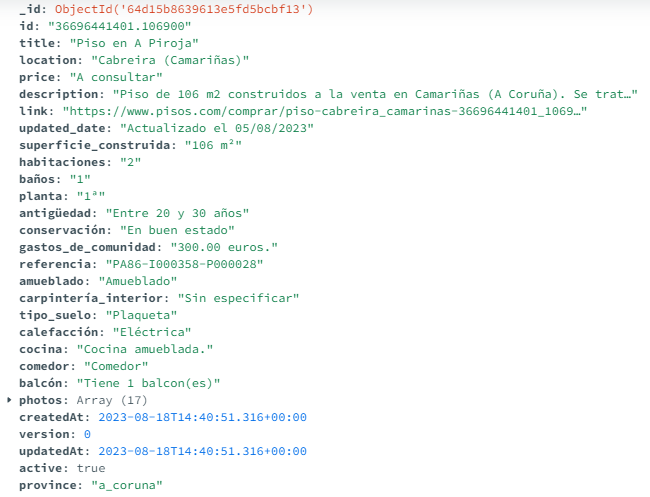
\includegraphics[width=1\textwidth]{img/documento_mongodb.PNG}
	\caption[Ejemplo de documento almacenado en base de datos MongoDB]{Ejemplo de documento almacenado en base de datos MongoDB que representa los datos de un inmueble en la colección ``a\_coruna''}
	\label{fig:documento_inmueble}
\end{figure}


\subsection{Datos en SQLite}

Tras un proceso de transformación los datos de la base de datos MongoDB se cargan en esta base de datos que consta principalmente de tres tablas:

\subsubsection{Tabla \texttt{last\_updated\_dates}}

Tabla operacional simple que almacena una columna con el nombre de la colección (de MongoDB) y otra con el tiempo de actualización (\texttt{updated\_at}) más reciente de dicha colección. Sirve para continuar el proceso de ETL en la siguiente iteración.

\subsubsection{Tabla \texttt{pisos}}{\label{subsec:tabla_pisos}}

Consta de los datos de inmuebles ya limpiados y transformados. Sirve tanto para el entrenamiento y predicción de los modelos de Aprendizaje Automático, como punto de partida de los datos agregados y para listar los inmuebles en el sitio web. 

Algunas columnas que merece la pena mencionar por su importancia operacional son: 

\begin{itemize}
\item \texttt{id} : Identificador único proveniente de pisos.com
\item \texttt{province} : La provincia del inmueble y por tanto su colección de MongoDB.
\item \texttt{capital} : Tiene valor 1 si pertenece a la capital de provincia, 0 si no.
\item \texttt{type} : Tipo de inmueble, por ejemplo Piso, Casa, Apartamento...
\item \texttt{price\_euro} : El precio de venta anunciado, incluye descuentos.
\item \texttt{link} : Enlace al inmueble en pisos.com.
\item \texttt{updated\_date} : Fecha actualización del anuncio reflejada en pisos.com.
\item \texttt{active} : Tiene valor 1 si el inmueble está considerado activo, 0 si no. Resultado del flujo de Scrapy que comprueba si el anuncio sigue activo.
\item \texttt{createdat} : Fecha de primera carga en MongoDB.
\item \texttt{updatedat} : Fecha de última actualización en MongoDB.
\item \texttt{version} : Indicador de cuantas veces se ha actualizado el inmueble en MongoDB.
\item \texttt{prediction} : Valor en € asignado por los modelos de Aprendizaje Automático.
\item \texttt{predictionupdatedat} : Tiempo en el que se actualizó el campo \texttt{prediction}.
\item \texttt{rating} : Valor calculado a través de \texttt{prediction} y \texttt{price\_euro}, explicado en \ref{sec:ml_section}). Sirve para ordenar los inmuebles de mayor a menor oportunidad.
\end{itemize}

En esta tabla, encontramos otros muchos campos que se pueden consultar en detalle en Tabla \ref{tab:schema_pisos}. Cabe mencionar que no todos los inmuebles presentan todos los campos, dependerá de cuales estén listados en el anuncio original, así encontramos muchos de ellos con valor \texttt{null}.

Finalmente, merece la pena mencionar que observamos algunos valores calculados que llevan el sufijo \texttt{\_summary} (marcado como \texttt{\_summ} en la tabla de referencia \ref{tab:schema_pisos}) o \texttt{\_cleaned}, estos datos son reagrupaciones de las mismas columnas sin sufijo que se pueden ver en la tabla, generalmente se trata de campos consolidados para su uso en los modelos. Se ha considerado que merece la pena mantener en la misma tabla los campos sin consolidar (más fieles al anuncio original) y consolidados.


\begin{longtable}{lll}
\caption{Esquema completo de la tabla \texttt{pisos}} \label{tab:schema_pisos} \\
\toprule
\textbf{Columna} & \textbf{Tipo} & \textbf{Desc.} \\
\midrule
\endfirsthead

\multicolumn{3}{c}%
{{\bfseries \tablename\ \thetable{} -- continuación de la página anterior}} \\
\toprule
\textbf{Columna} & \textbf{Tipo} & \textbf{Desc.} \\
\midrule
\endhead

\midrule
\multicolumn{3}{r}{{Continúa en la siguiente página}} \\
\endfoot

\bottomrule
\endlastfoot
id & TEXT & ID único \\
title & TEXT & Título \\
location & TEXT & Ubicación \\
province & TEXT & Provincia \\
capital & INTEGER & 0 No, 1 Yes \\
price\_euro & REAL & Precio € \\
description & TEXT & Descripción \\
link & TEXT & Enlace \\
updated\_date & TEXT & Fecha act. \\
sup.\_constr.\_m2 & REAL & Sup. constr. m² \\
sup.\_util\_m2 & REAL & Sup. útil m² \\
habitaciones & REAL & Habitaciones \\
banos & REAL & Baños \\
planta & TEXT & Planta \\
exterior & TEXT & Exterior \\
antiguedad & TEXT & Antigüedad \\
conservacion & TEXT & Conservación \\
referencia & TEXT & Ref. \\
terraza & TEXT & Terraza \\
photos & TEXT & Fotos \\
createdat & INTEGER & Creado \\
version & INTEGER & Versión \\
updatedat & INTEGER & Actualizado \\
active & INTEGER & Activo \\
amueblado & TEXT & Amueblado \\
armarios\_empotrados & TEXT & Armarios \\
tipo\_suelo & TEXT & Suelo \\
vidrios\_dobles & TEXT & Vidrios dobles \\
carpinteria\_exterior & TEXT & Carp. exterior \\
aire\_acondicionado & TEXT & Aire acond. \\
cocina & TEXT & Cocina \\
comedor & TEXT & Comedor \\
garaje & TEXT & Garaje \\
trastero & TEXT & Trastero \\
puerta\_blindada & TEXT & Puerta blindada \\
ascensor & TEXT & Ascensor \\
orientacion & TEXT & Orientación \\
soleado & TEXT & Soleado \\
chimenea & TEXT & Chimenea \\
piscina & TEXT & Piscina \\
gastos\_de\_comunidad & TEXT & Gastos com. \\
agua & TEXT & Agua \\
calefaccion & TEXT & Calefacción \\
old\_price\_euro & REAL & Precio antiguo € \\
sistema\_de\_seguridad & TEXT & Seguridad \\
balcon & TEXT & Balcón \\
superficie\_solar\_m2 & REAL & Sup. solar m² \\
tipo\_de\_casa & TEXT & Tipo de casa \\
urbanizado & TEXT & Urbanizado \\
calle\_alumbrada & TEXT & Calle alumbrada \\
calle\_asfaltada & TEXT & Calle asfaltada \\
portero\_automatico & TEXT & Portero autom. \\
adaptado\_movilidad\_reducida & TEXT & Adapt. movilidad \\
jardin & TEXT & Jardín \\
lavadero & TEXT & Lavadero \\
se\_aceptan\_mascotas & TEXT & Mascotas \\
telefono & TEXT & Teléfono \\
luz & TEXT & Luz \\
cocina\_equipada & TEXT & Cocina equip. \\
carpinteria\_interior & TEXT & Carp. interior \\
interior & TEXT & Interior \\
gas & TEXT & Gas \\
no\_se\_aceptan\_mascotas & TEXT & No mascotas \\
esquina & TEXT & Esquina \\
exterior\_summ & TEXT & Resumen exterior \\
vidrios\_dobles\_summ & TEXT & Resumen vidrios \\
adapt.\_mov.\_redu.\_summ & TEXT & Resumen adapt. movilidad \\
puerta\_blindada\_summ & TEXT & Resumen puerta blindada \\
ascensor\_summ & TEXT & Resumen ascensor \\
balcon\_summ & TEXT & Resumen balcón \\
portero\_automatico\_summ & TEXT & Resumen portero \\
garaje\_summ & TEXT & Resumen garaje \\
comedor\_summ & TEXT & Resumen comedor \\
terraza\_summ & TEXT & Resumen terraza \\
jardin\_summ & TEXT & Resumen jardín \\
armarios\_empotrados\_summ & TEXT & Resumen armarios \\
aire\_acondicionado\_summ & TEXT & Resumen aire acond. \\
trastero\_summ & TEXT & Resumen trastero \\
piscina\_summ & TEXT & Resumen piscina \\
chimenea\_summ & TEXT & Resumen chimenea \\
lavadero\_summ & TEXT & Resumen lavadero \\
urbanizado\_summ & TEXT & Resumen urbanizado \\
calle\_alumbrada\_summ & TEXT & Resumen calle alumbrada \\
calle\_asfaltada\_summ & TEXT & Resumen calle asfaltada \\
soleado\_summ & TEXT & Resumen soleado \\
gas\_summ & TEXT & Resumen gas \\
sistema\_de\_seguridad\_summ & TEXT & Resumen seguridad \\
interior\_summ & TEXT & Resumen interior \\
esquina\_summ & TEXT & Resumen esquina \\
amueblado\_summ & TEXT & Resumen amueblado \\
cocina\_equipada\_summ & TEXT & Resumen cocina equip. \\
mascotas\_summ & TEXT & Resumen mascotas \\
gastos\_de\_comunidad\_cleaned & REAL & Gastos com. limpios \\
carpinteria\_exterior\_cleaned & TEXT & Carp. exterior limpia \\
tipo\_suelo\_summ & TEXT & Resumen suelo \\
calefaccion\_summ & TEXT & Resumen calefacción \\
cocina\_summ & TEXT & Resumen cocina \\
orientacion\_summ & TEXT & Resumen orientación \\
agua\_summ & TEXT & Resumen agua \\
type & TEXT & Tipo \\
alcantarillado & TEXT & Alcantarillado \\
alcantarillado\_summ & TEXT & Resumen alcantarillado \\
prediction & REAL & Predicción \\
predictionupdatedat & TIMESTAMP & Fecha act. predicción \\
rating & REAL & Valoración \\
\end{longtable}
    
\subsubsection{Tabla \texttt{pisos\_dw}}{\label{subsec:pisos_dw}}

Esta tabla es el resultado del proceso de agregación de datos de la ETL, por lo tanto, se recalcula entera dos veces al día. Su objetivo principal es precalcular datos agregados para las visualizaciones, evitando la necesidad de computar estos datos en la web cada vez que el usuario haga una petición, como por ejemplo, al cambiar los filtros en la pestaña \textit{``VISUALIZA''}. Su origen único siempre es la tabla \texttt{pisos}.

Encontraremos todos los campos agrupados por:

\begin{itemize}
    \item \texttt{province\_group}: Provincia. Obtenido de \texttt{province} de tabla \texttt{pisos}.
    \item \texttt{capital\_group}: Si pertenecen a Capital de Provincia o no. Obtenido de \texttt{capital} de tabla \texttt{pisos}.
    \item \texttt{active\_group}: Si están en anuncios activos o no. Obtenido de \texttt{active} de tabla \texttt{pisos}.
    \item \texttt{updated\_month\_group}:  Mes-Año en el que se insertaron por primera vez en MongoDB (calculado desde campo \texttt{createdat} de tabla \texttt{pisos})
\end{itemize}

Además, para cada agrupación, existe un valor \texttt{'all'}, que identifica el cálculo sin tener en cuenta dicha agrupación. Por ejemplo, si todas las agrupaciones tienen valor \texttt{'all'} los cálculos agregados pertenecerán a todos los inmuebles de la base de datos, sin tener en cuenta provincia, capital, activos o tiempo de creación. 

Para algunas columnas provenientes de tabla \texttt{pisos}, denominadas como \textbf{numéricas} (Ver en Tabla \ref{tab:numerical_columns_pisosdw}), se calculan la media y la desviación estándar, descartando los \textit{outliers} para el cálculo.

El cálculo de \textit{outliers} se realiza teniendo en cuenta unos límites superiores e inferiores muy restrictivos, ya que no queremos eliminar muchos datos. Siendo $q1$ el cuartil 1, $q3$ el cuartil 3, e $iqr = q3 - q1$, los límites se definen como:

\begin{align*}
\text{Límite inferior} &= q1 - 5 \times iqr \\
\text{Límite superior} &= q3 + 5 \times iqr
\end{align*}

Para el resto de columnas provenientes de tabla \texttt{pisos}, denominadas como \textbf{categóricas} (Ver en Tabla \ref{tab:categorical_columns_pisosdw}), lo que se hace es calcular qué porcentaje de los inmuebles adquiere cada valor único posible, también siendo agrupados según los grupos mencionados previamente.

Por ejemplo para \texttt{piscina\_summary} los valores posibles son \texttt{YES} o \texttt{NO}. Se calculará que porcentaje de los inmuebles tienen cada uno de los valores, y se almacenarán dichos porcentajes en columnas distintas para cada valor único, que en este caso reciben el nombre de \texttt{piscina\_summary\_yes\_pct} y \texttt{piscina\_summary\_no\_pct}. Debemos tener en cuenta que estos porcentajes se calculan para cada combinación de agrupaciones, siendo así cada fila de la tabla una combinación distinta de agrupaciones.

\begin{table}[h]
\centering
\begin{tabular}{@{}ll@{}}
\toprule
\textbf{Columnas} & \\
\midrule
\texttt{price\_euro} & \texttt{superficie\_construida\_m2} \\
\texttt{superficie\_util\_m2} & \texttt{superficie\_solar\_m2} \\
\texttt{habitaciones} & \texttt{banos} \\
\texttt{gastos\_de\_comunidad\_cleaned} &  \\
\bottomrule
\end{tabular}
\caption[Columnas numéricas de la tabla \texttt{pisos} usadas para tabla agrupada \texttt{pisos\_dw}]{Columnas o campos numéricos de la tabla \texttt{pisos} usados para tabla agrupada \texttt{pisos\_dw}. Se muestran en dos grupos de columnas, para comprimir esta tabla.}
\label{tab:numerical_columns_pisosdw}
\end{table}

\begin{table}[h]
\centering
\begin{tabular}{@{}ll@{}}
\toprule
\textbf{Columnas} &  \\
\midrule
\texttt{exterior\_summary} & \texttt{comedor\_summary} \\
\texttt{vidrios\_dobles\_summary} & \texttt{terraza\_summary} \\
\texttt{adaptado\_...\_reducida\_summary} & \texttt{jardin\_summary} \\
\texttt{puerta\_blindada\_summary} & \texttt{armarios\_empotrados\_summary} \\
\texttt{ascensor\_summary} & \texttt{aire\_acondicionado\_summary} \\
\texttt{balcon\_summary} & \texttt{trastero\_summary} \\
\texttt{portero\_automatico\_summary} & \texttt{piscina\_summary} \\
\texttt{garaje\_summary} & \texttt{chimenea\_summary} \\
\texttt{lavadero\_summary} & \texttt{soleado\_summary} \\
\texttt{gas\_summary} & \texttt{amueblado\_summary} \\
\texttt{cocina\_equipada\_summary} & \texttt{calefaccion\_summary} \\
\texttt{conservacion} & \texttt{antiguedad} \\
\texttt{carpinteria\_exterior\_cleaned} & \texttt{tipo\_suelo\_summary} \\
\texttt{cocina\_summary} & \texttt{orientacion\_summary} \\
\bottomrule
\end{tabular}
\caption[Columnas categóricas de la tabla \texttt{pisos} usadas para tabla agrupada \texttt{pisos\_dw}]{Columnas o campos categóricos de la tabla \texttt{pisos} usados para tabla agrupada \texttt{pisos\_dw}. Se muestran en dos grupos de columnas, para comprimir esta tabla.}
\label{tab:categorical_columns_pisosdw}
\end{table}

\clearpage
\section{Diseño de Arquitectura de Software}

El diagrama de componentes se muestra en la Figura \ref{fig:arquitectura_general}. Englobando todos los componentes, encontramos un bloque en forma de elipse que representa la máquina virtual del proyecto. Este bloque a su vez contiene dos bloques rectangulares, uno que representa los servicios relacionados con los datos (\textit{Data Services}) y otro, los relacionados con la web (\textit{Web Services}). 

Dentro de estos bloques encontramos que cada contenedor de Docker se representa como un bloque con título en azul, cada volumen se representa con un bloque con título en morado. Encontramos las diferentes tareas (con sufijo \texttt{\_task}) englobando a distintos contenedores, y la frecuencia de la tarea se representa en un bloque con forma de nube.

\begin{figure} 
    \centering
    \begin{adjustbox}{center}
	    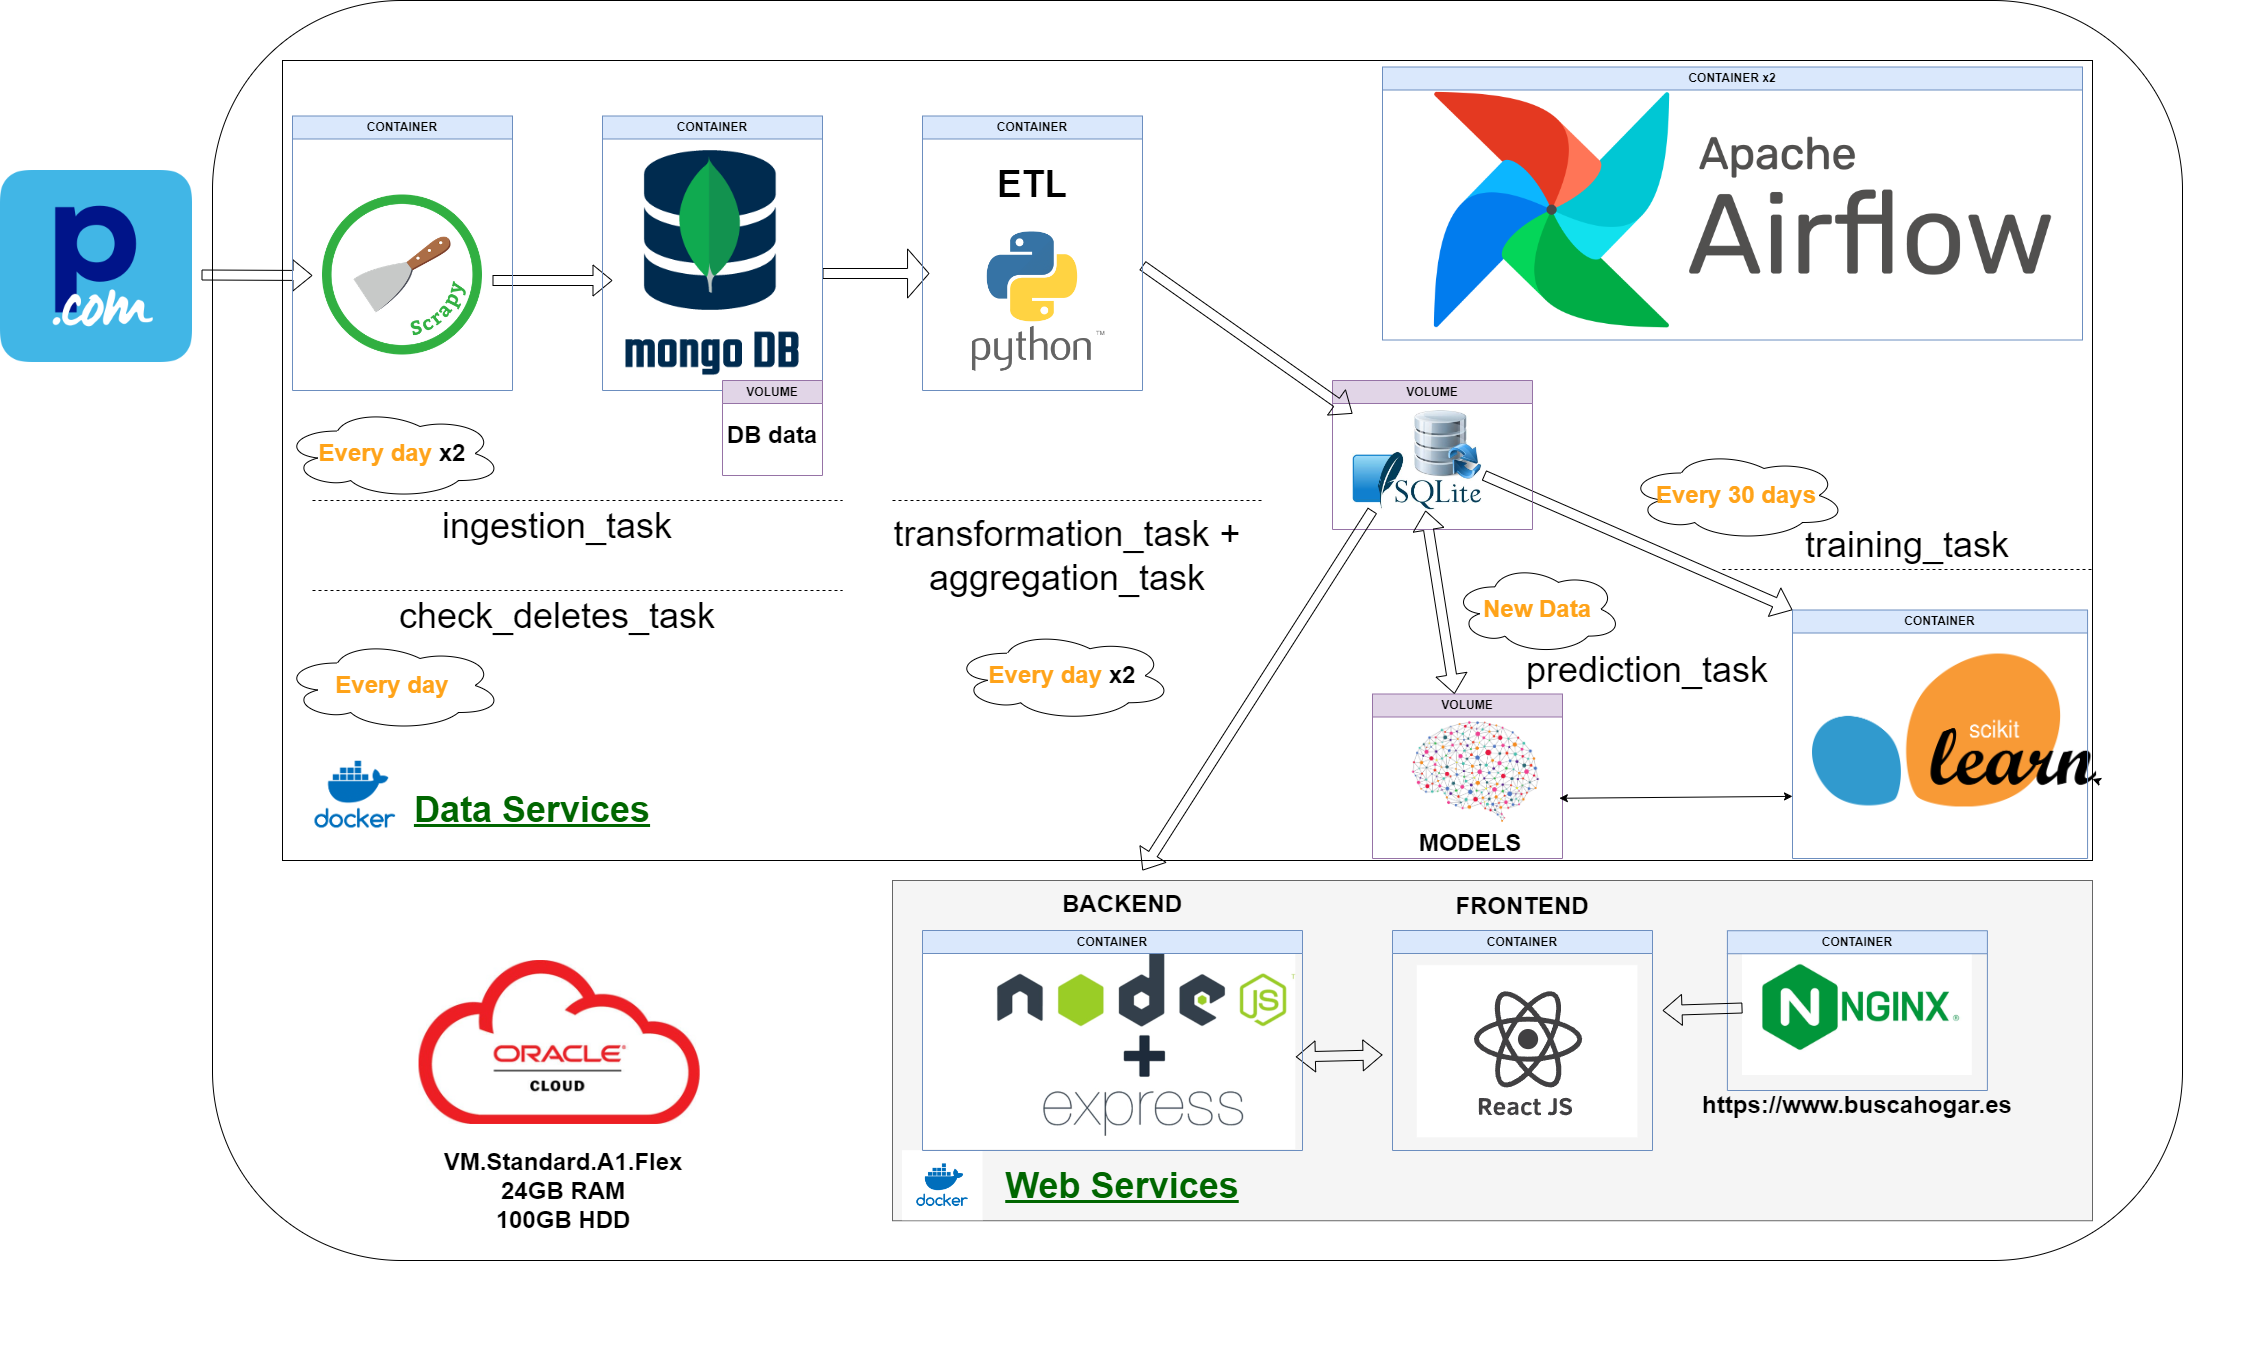
\includegraphics[width=1.1\textwidth]{img/arquitectura.png}
    \end{adjustbox}
    \caption{Arquitectura de software del proyecto}
    \label{fig:arquitectura_general}
\end{figure}
\clearpage 



\apendice{Documentación técnica de programación}

\section{Introducción}

El objetivo de este Apéndice es documentar a nivel técnico el presente proyecto, con objetivo de permitir la instalación en local del proyecto, facilitar el acceso a  un entorno de desarrollo y la extensión del proyecto.

\section{Estructura de directorios}

Todo el proyecto se ha desarrollando utilizando en un único repositorio \texttt{git} para control de versiones, que está disponible en el siguiente enlace: \url{https://github.com/dpuertamartos/big_data_tfm}.

Dentro del directorio raíz del repositorio, encontramos las carpetas mostradas en la Figura \ref{fig:dirtree_general} y además algunos archivos fundamentales para el proyecto. 

En la mayoría de las carpetas del repositorio, excepto \texttt{Latex}, \texttt{airflow} y \texttt{utils}, encontraremos un archivo con nombre \textit{Dockerfile}, que es el archivo de configuración del contenedor de Docker (Ver Sección \ref{sec:implementacion_docker}). En el servicio Airflow no es necesario dicho archivo, pues se usa una imagen oficial. En la carpeta \texttt{utils} simplemente se encuentra un \textit{script} que se corre periódicamente para renovar el certificado https, no siendo estrictamente necesario para el funcionamiento del proyecto.


\begin{figure}
	\dirtree{%
		.1 /big\_data\_tfm/ . 
            .2 Latex \textit{(Memoria del Proyecto)}.
            .3 img.
            .3 tex.
		.2 ETL \textit{(Servicio de ETL) \ref{sec:etl_section}}. 
            .2 ingestion\_scrapper \textit{(Servicio de scraping) \ref{sec:scrapy_section}}.
            .3 ingestion\_scrapper.
            .4 spiders.
            .4 fixes.
            .2 data\_analysis \textit{(Servicio de Aprendizaje Automático) \ref{sec:ml_section}}.
            .2 airflow \textit{(DAGs de Airflow) \ref{sec:airflow_section}}. 
            .3 dags.
            .2 backend \textit{(Backend del sitio web) \ref{sec:backend_section}}.
            .3 controllers.
            .3 requests.
            .3 util.
            .2 frontend \textit{(Frontend del sitio web) \ref{sec:frontend_section}}.
            .3 public.
            .3 src.
            .2 utils.
            .2 README.md \textit{(Documentación resumida)}.
            .2 architecture.drawio \textit{(Esquema de arquitectura)}.
            .2 docker-compose.yaml \textit{(Configuración de Docker Compose)}.
	}
	\caption{Árbol de directorios General}
	\label{fig:dirtree_general}
\end{figure}

\clearpage
\section{Manual del programador}

En esta sección se entrará más en detalle en como está estructurado y configurado el código, habrá una subsección para cada servicio (titulada con el nombre de la carpeta en el repositorio que aloja el código de dicho servicio) y una para las bases de datos.

Algunos aspectos generales que se mencionaran previamente para no repetirlos en cada subsección son los siguientes:

\begin{itemize}
    \item \texttt{requirements.txt}: Se tratan de archivos que describen las dependencias del servicio. Generados mediante el comando \texttt{pip freeze > requirements.txt}. Posteriormente se usan en el flujo de Docker para instalar dependencias. Usado para servicios que usan Python.
    \item \texttt{package.json}: Archivos de dependencias para los servicios web, gestionados por \texttt{npm}. Usado para servicios que usan Javascript (web).
    \item \texttt{Dockerfile}: Archivo de configuración de la imagen de Docker.
    \item \texttt{readme.md}: Archivos con documentación del servicio.
    \item Scripts shell (\texttt{.sh}): Actúan como vínculo entre el orquestador (Apache Airflow) y el propio servicio. Generalmente lanzan archivos \texttt{.py} y guardan \textit{logs}. Son ejecutados por el contenedor de Docker cuando este se lanza a través de Airflow.
\end{itemize}

\clearpage
\subsection{ingestion\_scrapper - Servicio de Scrapy}

Este servicio está escrito completamente en Python y sigue el esquema a creado tras ejecutar el comando \texttt{scrapy startproject ingestion\_scrapper}. En este proyecto los ficheros añadidos, modificados e inalterados respecto a la plantilla generada tras iniciar el proyecto, se muestran en la Figura \ref{fig:dirtree_scrapy}. Este servicio está pensado para funcionar con ejecuciones individualizadas, así, cada vez se lanza un contenedor de Docker que posteriormente se elimina. Con dicho contenedor, se puede lanzar tanto el servicio de recogida de datos de inmuebles (actualmente, 2 veces al día), como el servicio de comprobación de si los anuncios siguen activos (actualmente, 1 vez al día), según el \textit{Script} de Shell que lance.

Algunos detalles que merece la pena mencionar con los siguientes:

\begin{itemize}
    \item Carpeta \texttt{.../fixes/}: En esta carpeta se han recogido algunos scripts que se fueron utilizando a lo largo de los meses para adaptar el proyecto a nuevas funcionalidades. A día de hoy son prescindibles y no son necesarios para el funcionamiento del proyecto. Por ejemplo, encontramos un script \texttt{script\_to\_add\_active\_field.py}, que se usó para añadir el campo \texttt{active} a todos los inmuebles en la distintas colecciones de la MongoDB.
    \item Archivo \texttt{settings.py}: Desde aquí se modifica el comportamiento general de Scrapy
    \item Carpeta \texttt{.../spiders/}: Esta es la carpeta que realmente personaliza la funcionalidad del servicio de \textit{Scraping}. 
    
    Encontramos dos ``arañas'' distintas: una llamada \texttt{/spiders/pisos\_spider.py}, que es la que contiene toda la lógica para recopilar la información de inmuebles y otra,  \texttt{/spiders/check\_up\_spider.py}, que es la que contiene toda la lógica de verificar sin un anuncio sigue disponible o no.
    \item Los scripts de shell: \texttt{ingestion\_script.sh}, \texttt{ad\_up\_checking\_script.sh}. Son el punto único de enlace entre el orquestador y los dos tipos de tarea: La de recopilación/ingestión de inmuebles y la de comprobar si un anuncio sigue activo. Estos scripts generan logs que se almacenan en un volumen de Docker.
\end{itemize}


\begin{figure}
	\dirtree{%
		.1 /big\_data\_tfm/.
            .2 /ingestion\_scrapper/.
            .3 requirements.txt.
            .3 Dockerfile.
            .3 scrapy.cfg \textit{(Original)}.
            .3 /ingestion\_scrapper/.
            .4 /fixes/.
            .5 script...py \textit{(Scripts de uso único)}.
            .4 /spiders/.
            .5 \_\_init\_\_.py .
            .5 pisos\_spider.py \textit{(Añadido)}.
            .5 check\_up\_spider.py \textit{(Añadido)}.
            .4 \_\_init\_\_.py.
            .4 items.py \textit{(Original)}.
            .4 middlewares.py \textit{(Original)}.
            .4 pipelines.py \textit{(Original)}.
            .4 settings.py \textit{(Modificado)}.
            .4 config.py \textit{(Añadido)}.
            .4 ingestion\_script.sh \textit{(Añadido)}.
            .4 ad\_up\_checking\_script.sh \textit{(Añadido)}.
	}
	\caption{Árbol de directorios de servicio \textit{Scrapy}}
	\label{fig:dirtree_scrapy}
\end{figure}

\clearpage
\subsection{ETL}

Este servicio también está escrito completamente en Python, usando principalmente la librería Pandas~\cite{pandas}. Este servicio engloba dos tareas de las orquestadas por Airflow:

\begin{itemize}
    \item Transformación (ETL en sí): Lee de las colecciones de MongoDB y da lugar a la tabla \texttt{pisos} en SQLite (Ver subsección \ref{subsec:tabla_pisos}).
    \item Agregación: Lee de la tabla \texttt{pisos} y genera la tabla \texttt{pisos\_dw} (Ver subsección \ref{subsec:tabla_pisos}).
\end{itemize}

De igual forma que el servicio de \textit{Scrapy}, este servicio está pensado para funcionar con ejecuciones individualizadas, lanzando un contenedor de Docker que realizará una función según el \textit{Script} de Shell que lance. En la actualidad se ejecuta el servicio de transformación dos veces al día, seguido del de agregación. Se detallan los archivos en Figura \ref{fig:dirtree_ETL}.


\begin{figure}
	\dirtree{%
		.1 /big\_data\_tfm/.
            .2 /ETL/.
            .3 requirements.txt.
            .3 Dockerfile.
            .3 config.py.
            .3 aggregation.py \textit{(Principal Agregación)}.
            .3 extraction.py \textit{(ETL)}.
            .3 transformation.py \textit{(ETL)}.
            .3 transformation\_utils.py \textit{(ETL)}.
            .3 loading.py \textit{(ETL)}.
            .3 main.py \textit{(Principal ETL)}.
            .3 transformation\_script.sh \textit{(ETL)}.
            .3 aggregation\_script.sh \textit{(Agregación)}.
        }
	\caption{Árbol de directorios de servicio de ETL y Agregación}
	\label{fig:dirtree_ETL}
\end{figure}

\clearpage
\subsection{data\_analysis - Servicio de Aprendizaje Automático}

Este servicio se basa en el paquete \texttt{scikit learn}~\cite{scikit-learn} y está escrito en Python. Por una parte consta del código que entrena y genera los modelos, cuyo archivo principal es \texttt{train.py}, este utiliza funciones de \texttt{model\_generation.py}, y crea y almacena un ``limpiador/transformador'' final de los datos utilizando \texttt{data\_cleaning.py}. Este flujo de entrenamiento acaba con el almacenamiento permanente de los modelos y el ``limpiador'' en un volumen de Docker.

En el flujo de predicción, mucho más simple, encontramos solamente \texttt{generate\_predictions.py}. Este flujo carga los modelos y el limpiador de datos para aplicarlos las entradas más recientes de la tabla \texttt{pisos}.

Los datos se leen directamente de la tabla \texttt{pisos} de SQLite tanto para el entrenamiento (en este caso se leen datos de como máximo 6 meses de tiempo), como para el flujo de predicción de valor/puntuación, en este caso se leen los datos que aún no tienen predicción asignada.

Como entrada al código de Python, para cada uno de los dos flujos, encontramos de nuevo dos \textit{Scripts} de Shell: \texttt{predict.sh} y \texttt{train.sh}. Como pasaba para el servicio de \textit{Scrapy} y ETL, este servicio funciona con la construcción de un contenedor de Docker temporal, que llama a uno de estos dos \textit{Scripts} según la tarea y es orquestado por Airflow.

\begin{figure}
	\dirtree{%
		.1 /big\_data\_tfm/.
            .2 /data\_analysis/.
            .3 requirements.txt.
            .3 Dockerfile.
            .3 config.py.
            .3 convert\_db\_to\_csv.py
            .3 data\_cleaning.py.
            .3 model\_generation.py.
            .3 train.py.
            .3 generate\_predictions.py.
            .3 predict.sh \textit{(Regresión de Precio)}.
            .3 train.sh \textit{(Entrenamiento de modelos)}.
        }
	\caption{Árbol de directorios de servicio de Aprendizaje Automático}
	\label{fig:dirtree_ml}
\end{figure}

\clearpage
\subsection{airflow - Servicio de Airflow}

El servicio de Airflow se basa en la imagen \texttt{apache/airflow:2.7.1}. Así, se despliegan dos contenedores permanentes (a diferencia de los servicios anteriores), uno para \textit{webserver} (interfaz web de Airflow) y otro para \textit{scheduler}, para ver más detalles se puede ver el archivo \texttt{docker-compose.yaml} del proyecto.

Para iniciar correctamente el servicio por primera vez hay que seguir las instrucciones explicadas en Sección \ref{sec:instalacion_despliegue}.

Una vez en funcionamiento los contenedores y seguidas las instrucciones de instalación, los únicos archivos que encontramos en el proyecto son los relacionados con las DAGs~\cite{dags}, es decir los que indican las tareas a orquestar por Airflow, almacenados en \texttt{/big\_data\_tfm/airflow/dags/}. Estos archivos que configuran las DAGs se montan en los contenedores de Airflow.

Debemos tener en cuenta que todas las tareas de Airflow consisten en desplegar un contenedor de Docker temporal. Las podemos ver en Tabla \ref{table:dags}. Para más detalle se recomienda consultar el código de dichas DAGs.

\begin{table}[H]
\centering
\begin{tabular}{|l|l|l|}
\hline
\textbf{DAG} & \textbf{Frecuencia} & \textbf{Tareas} \\
\hline
\texttt{ingestion\_and\_ETL\_dag} & 2 por día & 
\texttt{ingestion\_task} \\
.py & & \texttt{checking\_deletes\_task} \textit{(1/día)} \\
& & \texttt{transformation\_task} \\
& & \texttt{aggregation\_task} \\
& & \texttt{prediction\_task} \\
\hline
\texttt{train\_dag.py} & 1 por mes & \texttt{training\_task} \\
& & \texttt{prediction\_task} \\
\hline
\texttt{mongo\_backup\_dag.py} & Cada 3 días & \texttt{mongo\_backup\_task} \\
\hline
\texttt{initial\_run\_dag.py} & Solo manual& Regenera el proyecto. \\
& & Utiliza una MongoDB restaurada \\
\hline
\end{tabular}
\caption{Descripción de las DAGs en Apache Airflow}
\label{table:dags}
\end{table}

\clearpage
\subsection{backend - Servicio \textit{Backend} de la Web}

Este servicio se compone de un servidor Node.js utilizando el framework Express, desarrollado completamente en JavaScript. El objetivo principal de este servicio es facilitar la comunicación entre la base de datos SQLite y la interfaz de usuario (\textit{Frontend}) del sitio web.

\paragraph{Arquitectura y Componentes Clave: } La arquitectura del servicio de backend está diseñada para ser modular, permitiendo una fácil expansión y mantenimiento (Ver Figura \ref{fig:dirtree_backend}). Los componentes clave incluyen:

\begin{itemize}
    \item \textbf{Controllers}: Carpeta \texttt{/controllers} contiene archivos como \texttt{flats.js} y \texttt{trends.js}, que definen las rutas de la API y los controladores asociados a ellas. Estos controladores procesan las peticiones entrantes, interactúan con la base de datos y devuelven las respuestas adecuadas al cliente.
    \item \textbf{Utilidades}: La carpeta \texttt{/util} incluye archivos cruciales como \texttt{config.js} para la configuración del entorno, \texttt{db.js} que maneja la conexión y operaciones de la base de datos, \texttt{logger.js} para el registro de actividades y errores, utilizado por middleware
    \texttt{middleware.js} que contiene middleware para manejo de errores, y \textit{logging}.
    \item \textbf{Configuración y Despliegue}: Archivos como \texttt{.dockerignore}, \texttt{.eslintrc.js}, y \texttt{.gitignore} configuran aspectos del entorno de desarrollo, \textit{linting} y versionado, respectivamente. \texttt{Dockerfile} permite la contenerización del servicio para un despliegue eficiente y consistente. 
    \item \textbf{Punto de Entrada}: \texttt{app.js} configura la aplicación Express, estableciendo middlewares y rutas principales, mientras que \texttt{index.js} sirve como el punto de entrada del servicio, iniciando el servidor y realizando configuraciones iniciales.
    \item \textbf{Gestión de Dependencias}: \texttt{package.json} y \texttt{package-lock.json} gestionan las dependencias del proyecto, asegurando versiones consistentes de las librerías y facilitando la instalación y actualización de paquetes.
\end{itemize}

\paragraph{Funcionamiento y Flujo de datos: }
Cuando una solicitud es recibida por el servidor, es procesada por el middleware correspondiente. Después, la solicitud es dirigida al controlador adecuado, donde se realizan operaciones específicas, como consultas o actualizaciones en la base de datos, antes de enviar una respuesta al cliente.

\begin{figure}
    \dirtree{%
        .1 /big\_data\_tfm/.
            .2 /backend/.
                .3 /controllers/.
                    .4 flats.js.
                    .4 trends.js.
                .3 /util/.
                    .4 config.js.
                    .4 db.js.
                    .4 logger.js.
                    .4 middleware.js.
                .3 .dockerignore.
                .3 .eslintrc.js.
                .3 .gitignore.
                .3 Dockerfile.
                .3 app.js.
                .3 index.js.
                .3 package.json.
                .3 package-lock.json.
    }
    \caption{Árbol de directorios del \textit{Backend} de la web}
    \label{fig:dirtree_backend}
\end{figure}


\subsection{frontend - Servicio \textit{Frontend} de la Web}

El servicio \textit{Frontend} está desarrollado utilizando React, una librería de JavaScript para construir interfaces web para el usuario. Se comunica con el servicio de \textit{Backend} para obtener y enviar datos, lo que permite a los usuarios interactuar con la información almacenada en la base de datos de forma intuitiva. La estructura del proyecto \textit{Frontend} se organiza según lo mostrado en la Figura \ref{fig:dirtree_frontend}.

En la carpeta \texttt{/public/} encontraremos recursos estáticos, imágenes e iconos que se usan en la aplicación. Dentro de la carpeta \texttt{/src/}, encontraremos las siguientes subcarpetas y archivos importantes:

\begin{itemize}
    \item \texttt{/assets/}: Contiene otros recursos estáticos
    \item \texttt{/components/}: Aquí se almacenan los componentes React, que son las unidades básicas de construcción de la interfaz de usuario. Cada componente (\texttt{.jsx}) representa una parte de la interfaz, como la página de inicio, la lista de pisos, las tendencias, el contacto y el pie de página. A su vez estas páginas están divididas en otros componentes
    \item \texttt{/services/}: Incluye servicios para la comunicación con el backend, como la obtención de datos de pisos y tendencias
    \item \texttt{/utils/}: Ofrece utilidades y funciones auxiliares, como opciones de selectores que son usadas a través de la aplicación
    \item \texttt{App.jsx}: El componente principal que engloba toda la aplicación React. En él se define la barra de navegación
    \item \texttt{index.css}: Hoja de estilos principal para la aplicación. No se ha utilizado demasiado, ya que se ha optado por dar la mayoría de los estilos dentro de los componentes.
    \item \texttt{main.jsx}: Punto de entrada de la aplicación React, donde se monta el componente principal \texttt{App}
\end{itemize}

Fuera de las carpetas \texttt{/public/} y \texttt{/src/}, encontramos varios archivos y configuraciones relevantes para el proyecto:

\begin{itemize}
    \item \texttt{.dockerignore}, \texttt{.eslintrc.js}, \texttt{.gitignore}: Archivos de configuración para Docker, ESLint y Git, respectivamente, que ayudan a gestionar el entorno de desarrollo y control de versiones.
    \item \texttt{Dockerfile}: Define las instrucciones para crear una imagen Docker del servicio 
    \item \texttt{package.json} y \texttt{package-lock.json}: Estos archivos gestionan las dependencias del proyecto, especificando las librerías y paquetes necesarios para el desarrollo y ejecución de la aplicación.
    \item \texttt{vite.config.js}: Configuración de Vite~\cite{vite} específica para este proyecto, optimizando el proceso de construcción y desarrollo.
    \texttt{provinces.json}: Un archivo de datos utilizado por la aplicación, datos estáticos.
\end{itemize}

Utilizando Vite~\cite{vite}, un paquete para crear rápidamente plantillas para aplicaciones React, este proyecto \textit{Frontend} aprovecha una compilación rápida y un servidor de desarrollo eficiente con autorecarga cuando se cambia algún componente, lo que resulta en una mejora significativa en la velocidad de desarrollo.

\begin{figure}
    \dirtree{%
        .1 /big\_data\_tfm/.
            .2 /frontend/.
                .3 /public/.
                    .4 flats.jpg.
                    .4 favicon.ico.
                .3 /src/.
                    .4 /assets/.
                        .5 react.svg.
                    .4 /components/.
                        .5 Home.jsx.
                        .5 Flats.jsx.
                        .5 Trends.jsx.
                        .5 Contact.jsx.
                        .5 Footer.jsx.
                        .5 ....jsx.
                    .4 /services/.
                        .5 flats.js.
                        .5 trends.js.
                    .4 /utils/.
                        .5 selector\_options.js.
                    .4 App.jsx.
                    .4 index.css.
                    .4 main.jsx.
                .3 .dockerignore.
                .3 .eslintrc.js.
                .3 .gitignore.
                .3 Dockerfile.
                .3 index.html.
                .3 index.js.
                .3 package.json.
                .3 package-lock.json.
                .3 vite.config.js.
                .3 README.md.
                .3 provinces.json.
                }
    \caption{Árbol de directorios del \textit{Frontend} de la web}
    \label{fig:dirtree_frontend}
\end{figure}

\clearpage
\subsection{Bases de datos: MongoDB y SQLite}

\paragraph{La base de datos MongoDB: }Su elección y utilidad se explica en la Sección \ref{sec:mongodb_section}, funciona con un contenedor de Docker que utiliza la última imagen disponible \texttt{mongo:latest}, y almacena los datos en un volumen (\texttt{mongodb-data}) montado en el contenedor. No necesita ningún tipo de instalación más que seguir el procedimiento de la Sección \ref{sec:instalacion_despliegue}

En el archivo \texttt{/big\_data\_tfm/readme.md}, existe una sección titulada \texttt{6. MongoDB} donde se explica como restaurar un \textit{backup} de mongodb. Estos \textit{backups} se generan cada 3 días si se activa el DAG \texttt{mongo\_backup\_dag.py} (Ver Tabla \ref{table:dags}). Para mover dicho \textit{backup} del volumen \texttt{\{project\}\_mongodb-backups} al sistema de archivos local se puede seguir la sección titulada \texttt{8. DEV-UTILS} del archivo \texttt{readme.md.}

Esta base de datos es la clave del proyecto, y utilizando un \textit{backup} de la misma, se puede regenerar la base de datos SQLite, los modelos y continuar con el proceso de \textit{scraping} desde un punto anterior, aunque hayan pasado múltiples días/semanas e incluso meses sin actualización.

\paragraph{La base de datos SQLite: } Se trata únicamente de un archivo nombrado \texttt{pisos.db}, que se genera por primera vez, si no existe, tras ejecutar la tarea de ETL. Este archivo se almacena en un volumen de Docker que se monta en los distintos contenedores (Ver archivo \texttt{docker-compose.yaml} y observar volumen nombrado como \texttt{sqlite-db}).

Es extremadamente sustituible, esta base de datos completa se puede regenerar en pocos minutos a partir de una copia de la base de datos MongoDB, por ello no se realizan \textit{backups}. Su mayor utilizad es dar rápido acceso a datos estructurados/tabulares por la web y los tareas de Aprendizaje Automático.

\clearpage
\section{Compilación, instalación y ejecución del proyecto}\label{sec:instalacion_despliegue}

En esta sección se abordará como ejecutar el proyecto completo en un entorno local. Aunque el proyecto está desplegado en una máquina virtual de Oracle Cloud, podría ser desplegado en cualquier máquina de forma similar, incluida la web.

Solo se abordará la ejecución mediante Docker, ya que es la única solución unificada. Sin embargo, sería totalmente posible la instalación y ejecución de cada uno de los servicios sin utilizar ningún tipo de contenedor, aunque no está explicada ni soportada en esta memoria por su extensión. Cabe señalar que hay mucha información ampliada en el archivo \texttt{/big\_data\_tfm/readme.md}, disponible para consulta si se quieren más detalles.

Los prerequisitos son los siguientes:

\begin{itemize}
    \item Docker instalado
    \item Terminal Unix (Compatible WSL de Windows)
    \item Dar permisos de escritura y lectura en el socket de Docker para todos los usuarios. Esto es necesario para que Airflow utilice el socket. 
    
    \texttt{sudo chmod 666 /var/run/docker.sock}
    
\end{itemize}

A continuación necesitamos completar algunos pasos imprescindibles, antes de tener el proyecto en funcionamiento:

\begin{itemize}
    \item Clonar repositorio

    \texttt{git clone https://github.com/dpuertamartos/big\_data\_tfm.git}

    \item Iniciar la base de datos de Airflow

    \texttt{docker-compose run --rm airflow\_webserver airflow db init}

    \item Crear usuario para Airflow. Por defecto, usuario \texttt{admin}, password \texttt{admin}.

\begin{lstlisting}
docker-compose run \
--rm airflow_webserver airflow \
users create \
--username admin \
--firstname FIRST_NAME \
--lastname LAST_NAME \
--role Admin \
--email admin@example.org \
--password admin 
\end{lstlisting}

    \item Construir contenedores para \textit{Scraping}, ETL y Aprendizaje Automático. Estos contenedores son lanzados y destruidos tras cada ejecución, no están continuamente activos.

    \texttt{docker-compose build scraper etl data\_analysis}

    \item Lanzar contenedores para Airflow, Mongodb y la web

    \texttt{docker-compose up -d mongodb airflow\_webserver airflow\_scheduler app backend nginx}

    Se debe tener en cuenta que la web en local no mostrará datos hasta que pasen unos días con el servicio de ingestión o bien se regeneren las bases de datos a partir de un \textit{backup} (Explicado en subsección \ref{sec:regenerar_desde_backup}).

    \item Acceder a interfaz de Airflow en el Navegador \texttt{http://0.0.0.0:8080/}:
    
    Como mínimo se debe activar la DAG \texttt{ingestion\_transformation\_dag}, que iniciará la recogida de datos. 
    
    Se recomienda activar \texttt{training\_dag}, solo si ya se tienen unas semanas de recogida de datos o si se ha partido de un \textit{backup} de MongoDB y se ha lanzado ya \texttt{initial\_run\_dag}.

    Opcionalmente podemos activar \texttt{mongo\_backup\_dag} si queremos que se realice un backup del volumen que contiene los datos de MongoDB cada tres días.

    En la Figura \ref{fig:airflow_interfaz} se pueden ver las DAGs activadas en una ejecución del producto madurada durante varios meses. 
\end{itemize}

\begin{figure}[ht]
    \centering
	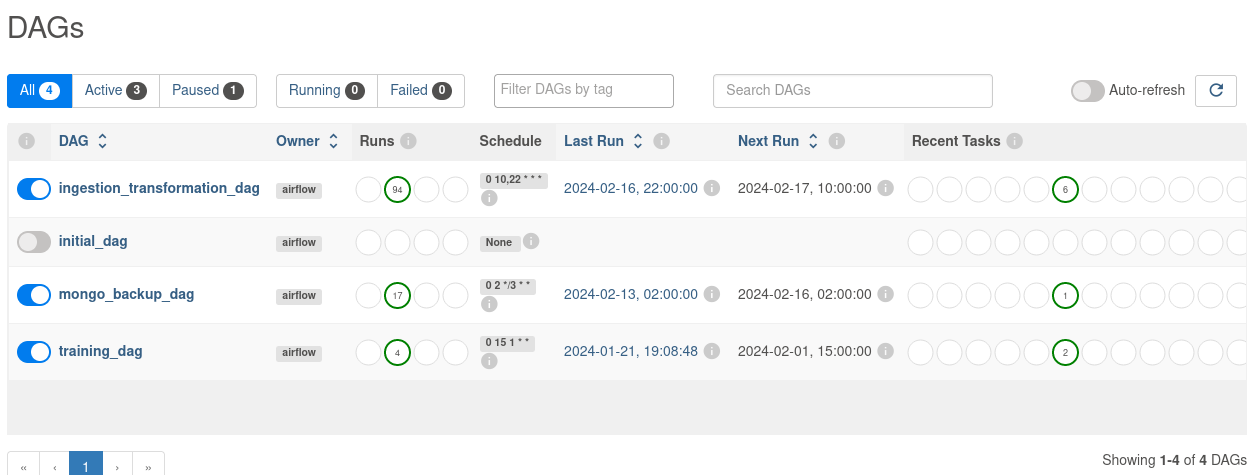
\includegraphics[width=1\textwidth]{img/airflow_interfaz.PNG}
	\caption[Interfaz de Apache Airflow Web Server, con DAGs del proyecto]{Interfaz de Apache Airflow Web Server, con DAGs del proyecto activadas en la máquina del entorno de producción. Se activan pulsando el \textit{slider} azul/gris a la izquierda del nombre.}
	\label{fig:airflow_interfaz}
\end{figure}

\clearpage
\section{Cómo regenerar todo el proyecto desde un \textit{backup} de MongoDB}\label{sec:regenerar_desde_backup}

Primero, debemos restaurar los datos en MongoDB, el proceso de recuperación dependerá de como se ha generado el \textit{backup}. Si se trata de un \textit{backup} generada a través de la DAG de este proyecto destinada a tal causa, seguiremos los siguientes pasos después de clonar el repositorio (Se deben cumplir los prerrequisitos de la Sección \ref{sec:instalacion_despliegue}):

\begin{itemize}

    \item Si existe un volumen previo con datos de MongoDB, lo borramos

    \texttt{docker volume remove big\_data\_tfm\_mongodb-data}
    
    \item Iniciamos el contenedor de MongoDB, creando el volumen de datos asociado:
    
    \texttt{docker compose up -d mongo}
    
    \item Descomprimiremos el \textit{backup} obteniendo una carpeta denominada \textit{mongo\_backup} o similar

    \item Copiaremos el \textit{backup} dentro de una carpeta temporal del contenedor

    \texttt{docker cp /path/to/backup/mongo\_backup/ mongodb-container:/tmp/bkup}

    \item Restauraremos el \textit{backup} con el siguiente comando

    \texttt{docker exec -it mongodb-container mongorestore /tmp/bkup}

    \item Eliminamos la carpeta temporal del contenedor

    \texttt{docker exec mongodb-container rm -rf /tmp/bkup}
    
    
\end{itemize}

Posteriormente continuaremos con los pasos de la sección \ref{sec:instalacion_despliegue} y al llegar al apartado de iniciar las DAGs, deberemos activar manualmente la DAG \texttt{initial\_run\_dag} una sola vez, esto regenerará la base de datos SQLite y se entrenaran los modelos (Puede tardar un par de horas según la máquina). Finalmente, tras el éxito de regenerar el resto de elementos a partir del \textit{backup} de MongoDB, ya podemos activar las DAGs como aparece en la Figura \ref{fig:airflow_interfaz}, tendremos todos los servicios orquestados y la web disponible con los datos hasta el punto que tuviese almacenado el \textit{backup}.

\apendice{Documentación de usuario}

\section{Introducción}

En este Apéndice se resumirá como interaccionar con la interfaz web que da acceso al conjunto de datos curado.

\section{Requisitos e Instalación}

Al tratarse de una aplicación web al uso, el usuario simplemente debe acceder con cualquier navegador con JavaScript activo (Chrome, Firefox, Edge...) al dominio \href{https://www.buscahogar.es}{buscahogar.es}.

\clearpage
\section{Manual del usuario}

En esta sección se detallará como interactuar con las distintas vistas del sitio web: \texttt{INICIO}, \texttt{EXPLORA}, \texttt{VISUALIZA} e \texttt{INFO}. Tras acceder a la página, lo que vemos se observa en la Figura \ref{fig:inicio_0}



Se puede acceder a las distintas vistas del sitio web a través de la barra de navegación, mostrada en la parte superior derecha de la Figura~\ref{fig:inicio_0}. En dicha barra de navegación, la vista seleccionada se remarca en color azul.

\begin{figure}[ht]
    \centering
	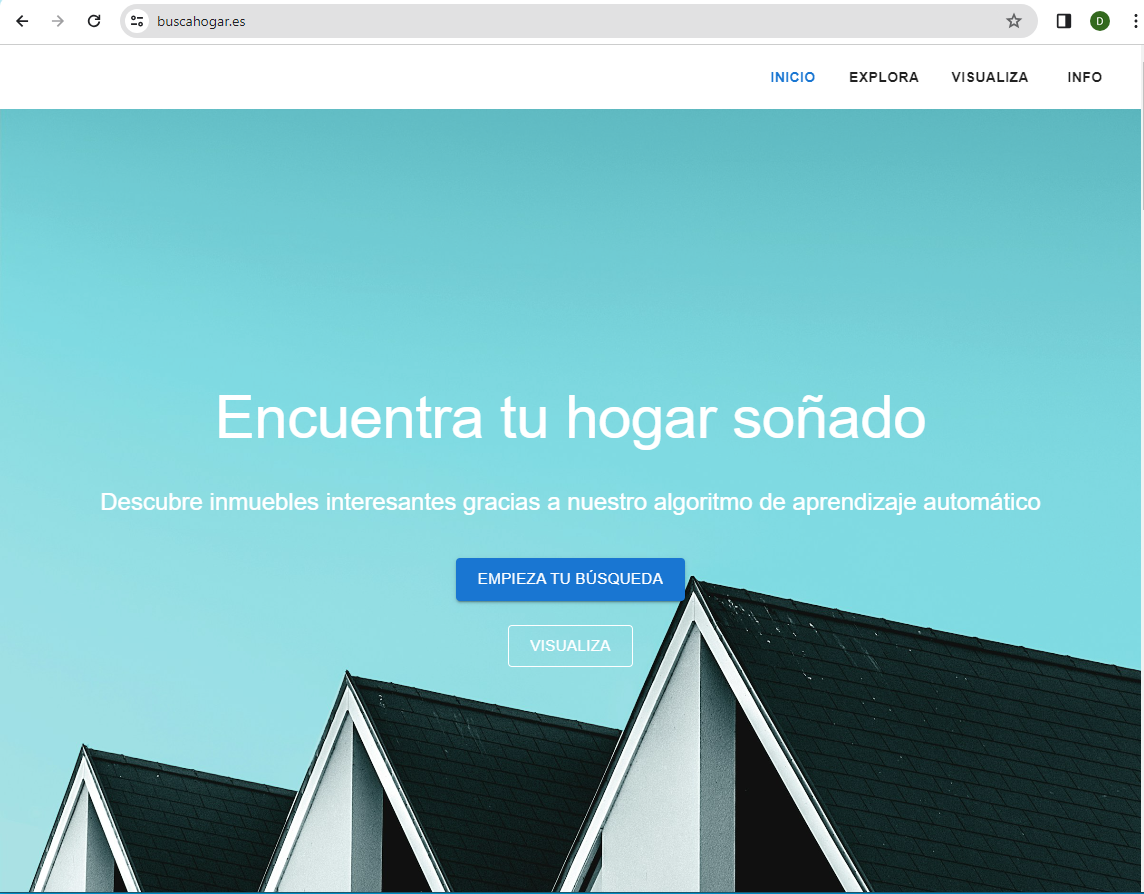
\includegraphics[width=1\textwidth]{img/inicio_0.PNG}
	\caption[Página de inicio \url{www.buscahogar.es}]{Página de inicio \url{www.buscahogar.es}, en la parte superior derecha vemos la barra de navegación}
	\label{fig:inicio_0}
\end{figure}

\begin{figure}[ht]
    \centering
	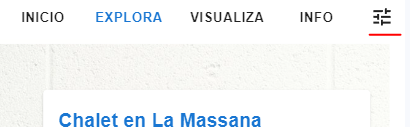
\includegraphics[width=1\textwidth]{img/filtro_replegado_1.PNG}
	\caption[Barra de navegación de \url{www.buscahogar.es} en pantallas móviles]{Barra de navegación de \url{www.buscahogar.es} en pantallas móviles. Al pulsar el botón marcado en rojo se despliegan los filtros de las pestañas \texttt{INICIO}, \texttt{EXPLORA} y \texttt{VISUALIZA}.}
	\label{fig:filtro_moviles}
\end{figure}

\clearpage
\subsection{INICIO}{\label{sec:web_inicio}}

En esta vista se muestra la página de inicio, que hace la función de ventana de \textit{marketing} para el resto del portal. Tras unos breves textos de ``llamada a la acción'', encontramos una sección con funcionalidad que merece la pena explicar (Ver Figura \ref{fig:inicio_1}): 

En esta sección se muestran los inmuebles con mayor puntuación asignada por los modelos para las provincias seleccionadas (Ver calculo en Sección \ref{sec:ml_section}). Por defecto, aparecen los cinco inmuebles de mayor puntuación para todas las provincias y además, el modo inteligente (\textit{Smart Mode}) se encuentra  activado. Este modo limita la puntuación máxima a 0.4 (Lo que significa que los modelos le asignan un 40\% más de precio que el de venta), ya que se ha observado que inmuebles con más de esa puntuación suelen ser falsos positivos.

Por lo tanto, encontramos tres selectores: (1) Provincia, (2) Si queremos inmuebles solo en capital de provincia, (3) Modo Inteligente (limitación a 0.4 de puntuación máxima). Además, encontramos botón de interrogación que explica en qué consiste el modo inteligente. Estos selectores se repliegan en pantallas móviles, para desplegarlos hay que pulsar el icono de filtro en la parte superior derecha (ver Figura \ref{fig:filtro_moviles}).


\begin{figure}[ht]
    \centering
	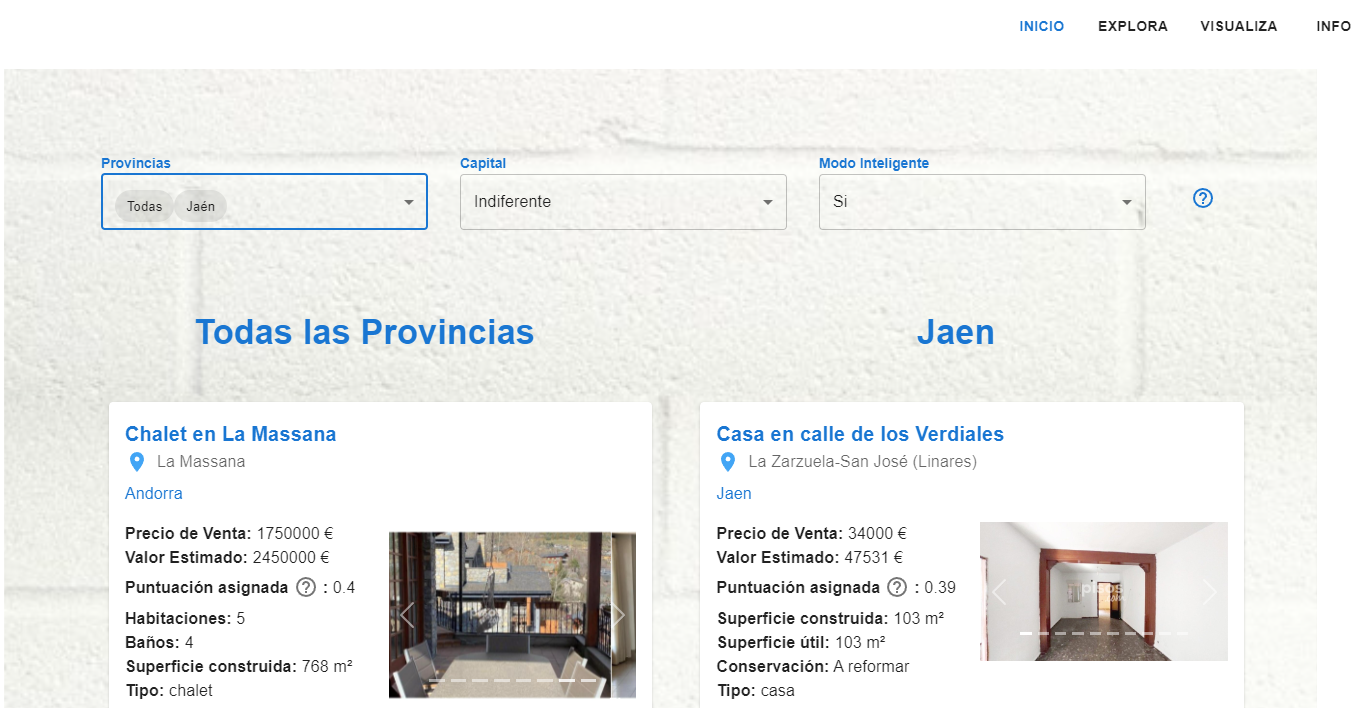
\includegraphics[width=1\textwidth]{img/inicio_1.PNG}
	\caption[Parte inferior de la página de INICIO en \url{www.buscahogar.es}]{Parte inferior de la página de INICIO en \url{www.buscahogar.es} con provincia ``Todas'' y ``Jaen'' seleccionadas}
	\label{fig:inicio_1}
\end{figure}

\clearpage
\subsection{EXPLORA}{\label{sec:web_explora}}

En esta sección, que representa el núcleo de la web, encontramos el acceso al listado de todos los inmuebles en la base de datos. En la parte izquierda encontramos los filtros y en la derecha el listado de inmuebles (Ver Figura \ref{fig:explora_1}. En pantallas móviles o de pequeño tamaño, los filtros de la parte izquierda se repliegan, para desplegarlos hay que pulsar el icono de filtro en la parte superior derecha (Ver Figura \ref{fig:filtro_moviles}).

Por defecto, los inmuebles están organizados en orden de puntuación descendente, con un máximo de 0.4 (equivalente al modo Inteligente, explicado en Sección \ref{sec:web_inicio}. Todos los inmuebles listados incluyen los datos originales listados en \url{www.pisos.com}, y además el valor estimado por los modelos de Aprendizaje Automático, junto con la puntuación (Para ver como se calcula ver \ref{sec:ml_section}), además de un botón con forma de interrogación que explica la puntuación asignada.

Los filtros, desde la parte superior a la inferior, son los siguientes:

\begin{itemize}
    \item Provincia: La Provincia de la que quieres ver inmuebles
    \item Capital: Si quieres ver inmuebles solo en la capital de Provincia, fuera de la capital o indiferente.
    \item Tipo: El tipo de inmueble, puede ser indiferente. Piso, casa, apartamento...
    \item Precio (\textit{Slider}): El rango de precios (en €) que queremos ver. Se trata del precio de venta real del inmueble.
    \item Habitaciones (\textit{Slider}): Los inmuebles que se mostrarán estarán en ese rango de número de habitaciones que queremos ver.
    \item M2 Útiles (\textit{Slider}):  Los inmuebles que se mostrarán estarán en ese rango de metros cuadrados útiles que queremos ver.
    \item Puntuación (\textit{Slider}): Los inmuebles que se mostrarán estarán en ese rango de puntuaciones (asignadas por Aprendizaje Automático)
    \item Ordenar por: La forma en la que quieres ordenar el listado, por defecto en puntuación descendente. 
\end{itemize}

De forma interesante, la pestaña explora no incorpora paginación como suele ocurrir en los portales inmobiliarios comunes, se ha implementado un mecanismo de \textit{scroll} infinito similar al de la mayoría de redes sociales, en el que se van cargando inmuebles que cumplen las especificaciones del filtro a medida que el usuario alcanza el límite inferior de la página.

\begin{figure}[ht]
    \centering
	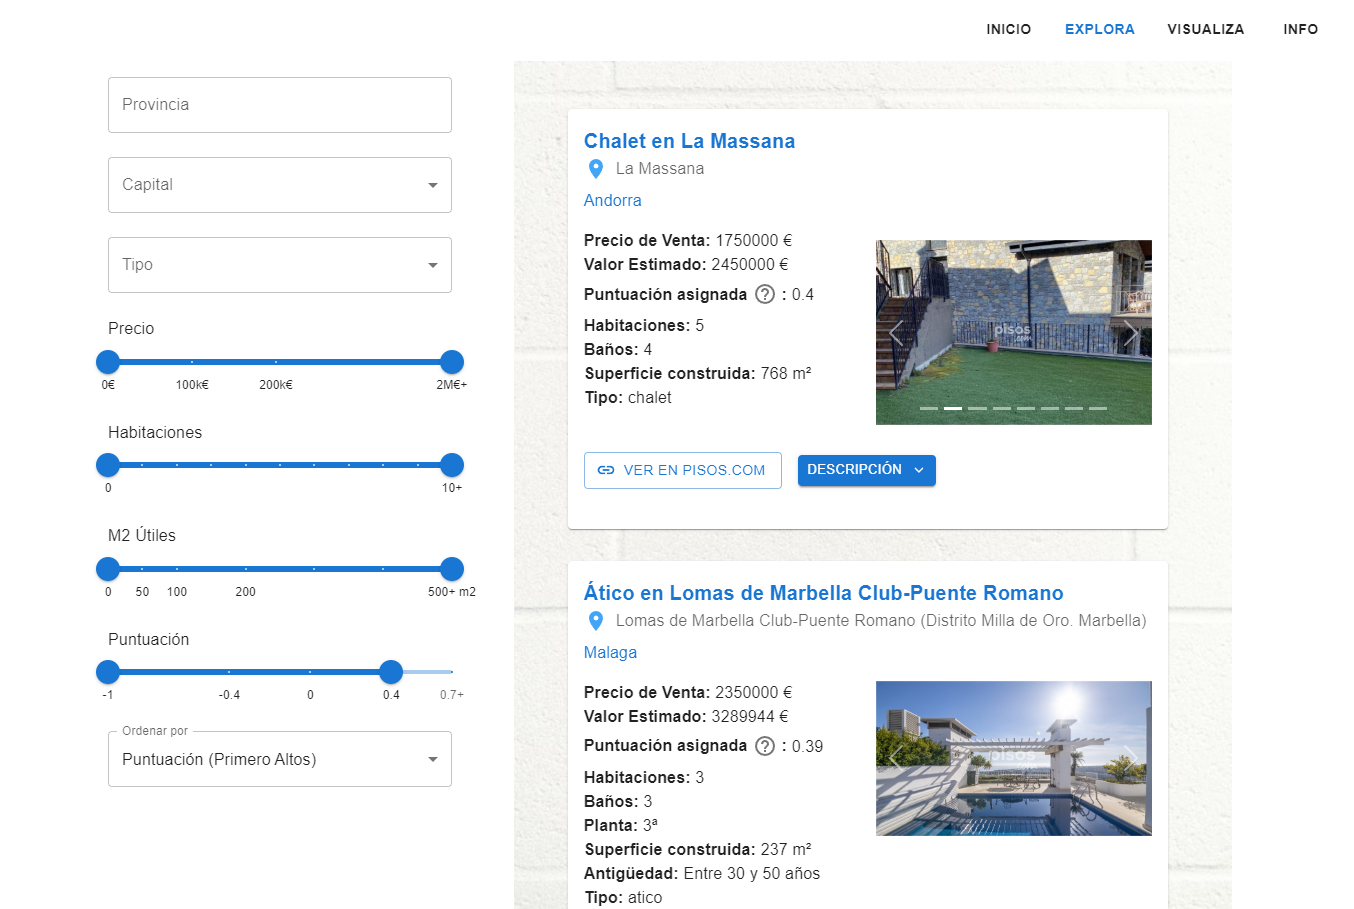
\includegraphics[width=1\textwidth]{img/explora_1.PNG}
	\caption{Vista general de página EXPLORA en \url{www.buscahogar.es}}
	\label{fig:explora_1}
\end{figure}

\clearpage
\subsection{VISUALIZA}{\label{sec:web_visualiza}}

Esta pestaña es la zona de visualización de los datos agregados en la tabla explicada en el Apéndice \ref{subsec:pisos_dw}.

Se presentan tres zonas claramente diferenciadas, una superior con filtros para las gráficas, una media con gráfica(s) de líneas y una inferior con un gráfico de barras y un mapa. En pantallas móviles o de pequeño tamaño, los filtros superiores se repliegan, para mostrarlos hay que pulsar el icono de filtro en la parte superior derecha (Ver Figura \ref{fig:filtro_moviles}).

Los filtros son los siguientes:

\begin{itemize}
    \item Comunidad Autónoma (CA): La CA de la que se quieren ver datos. Al seleccionarla, automáticamente se seleccionan todas las Provincias de dicha CA. Selección múltiple
    \item Provincia: La Provincia de la que se quieren ver inmuebles. Selección múltiple.
    \item Capital: Si se quieren ver inmuebles solo en la capital de Provincia, fuera de la capital o indiferente.
    \item Tipo: El tipo de inmueble, puede ser indiferente. Piso, casa, apartamento...
    \item Activo: Si se quieren datos de anuncios activos, retirados/vendidos o indiferente.
\end{itemize}

En la gráficas de líneas muestran datos promediados (eje $Y$), denominados como \texttt{Medidas} en la interfaz. Se observa la evolución de dichas medidas a lo largo de los meses (eje $X$). Como máximo se pueden seleccionar tres a la vez, mostrándose tres gráficas de líneas, en las que cada línea es una CA/Provincia/Media Total. Dichos datos son los siguientes actualmente:

\begin{itemize}
    \item Precio (€)
    \item Superficie útil ($m^2$)
    \item Superficie de solar ($m^2$)
    \item Número de habitaciones (ud)
    \item Número de baños (ud)
    \item Gastos de comunidad (€)
    \item Cantidad de inmuebles (anuncios) en venta / extraídos (ud)
    \item Precio por Metro Cuadrado (€)
    \item Precio por Habitación (€)
    \item Precio por Baño (€)
\end{itemize}

En la parte inferior del gráfico (parte denominada como ``categórica''), se muestran (en \%), los valores que toman las categorías seleccionadas. 


Por ejemplo, si seleccionamos categoría \texttt{Piscina Sí (\%)} se nos muestra el \% de inmuebles de cada comunidad/provincia/media total que tienen Piscina (Ver Figura \ref{fig:visualiza_1}). En el gráfico de barras se muestra una barra con el porcentaje, y en el mapa aparece un círculo localizado en dicha provincia con área proporcional al porcentaje. Si se ha seleccionado una comunidad autónoma, en el gráfico de barras aparece la media de la comunidad autónoma y en el mapa todas las provincias de dicha comunidad autónoma.


\begin{figure}[ht]
    \centering
	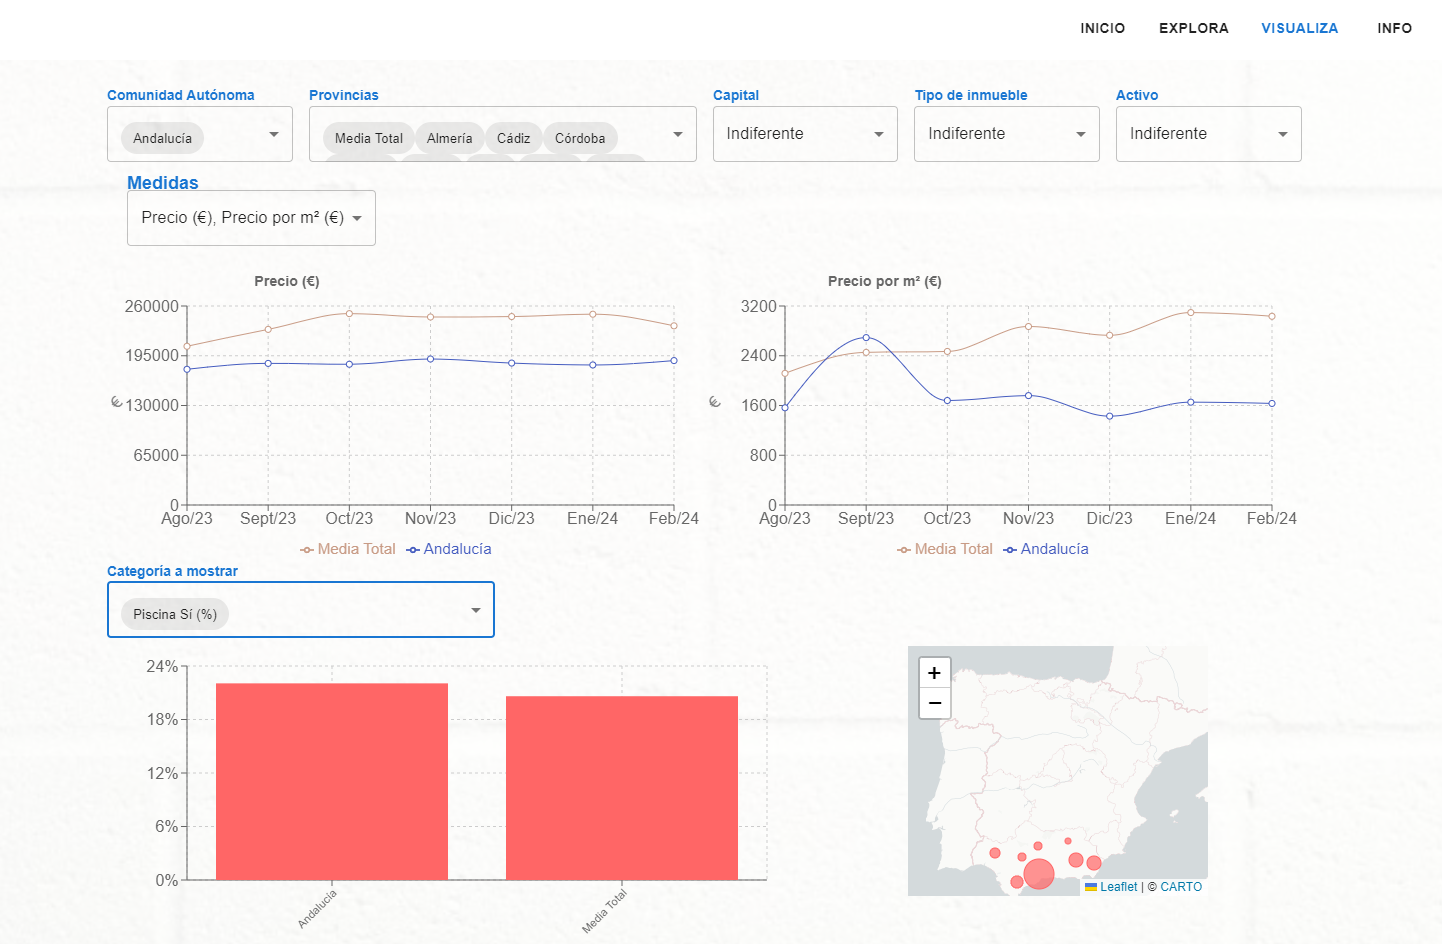
\includegraphics[width=1\textwidth]{img/visualiza_1.PNG}
	\caption[Vista general de página VISUALIZA en \url{www.buscahogar.es}]{Vista general de página VISUALIZA en \url{www.buscahogar.es}. Se ha seleccionado la comunidad autónoma Andalucía, y la categoría a mostrar \texttt{Piscina Si (\%)}}
	\label{fig:visualiza_1}
\end{figure}


\subsection{INFO}{\label{sec:web_info}}

Se trata de una sección de contacto, con el e-mail del autor principal del presente proyecto y algunas preguntas y respuestas frecuentes.




\bibliographystyle{plain}
\bibliography{bibliografia}

\end{document}
